\documentclass[11pt]{article}

    \usepackage[breakable]{tcolorbox}
    \usepackage{parskip} % Stop auto-indenting (to mimic markdown behaviour)
    
    \usepackage{iftex}
    \ifPDFTeX
    	\usepackage[T1]{fontenc}
    	\usepackage{mathpazo}
    \else
    	\usepackage{fontspec}
    \fi

    % Basic figure setup, for now with no caption control since it's done
    % automatically by Pandoc (which extracts ![](path) syntax from Markdown).
    \usepackage{graphicx}
    % Maintain compatibility with old templates. Remove in nbconvert 6.0
    \let\Oldincludegraphics\includegraphics
    % Ensure that by default, figures have no caption (until we provide a
    % proper Figure object with a Caption API and a way to capture that
    % in the conversion process - todo).
    \usepackage{caption}
    \DeclareCaptionFormat{nocaption}{}
    \captionsetup{format=nocaption,aboveskip=0pt,belowskip=0pt}

    \usepackage{float}
    \floatplacement{figure}{H} % forces figures to be placed at the correct location
    \usepackage{xcolor} % Allow colors to be defined
    \usepackage{enumerate} % Needed for markdown enumerations to work
    \usepackage{geometry} % Used to adjust the document margins
    \usepackage{amsmath} % Equations
    \usepackage{amssymb} % Equations
    \usepackage{textcomp} % defines textquotesingle
    % Hack from http://tex.stackexchange.com/a/47451/13684:
    \AtBeginDocument{%
        \def\PYZsq{\textquotesingle}% Upright quotes in Pygmentized code
    }
    \usepackage{upquote} % Upright quotes for verbatim code
    \usepackage{eurosym} % defines \euro
    \usepackage[mathletters]{ucs} % Extended unicode (utf-8) support
    \usepackage{fancyvrb} % verbatim replacement that allows latex
    \usepackage{grffile} % extends the file name processing of package graphics 
                         % to support a larger range
    \makeatletter % fix for old versions of grffile with XeLaTeX
    \@ifpackagelater{grffile}{2019/11/01}
    {
      % Do nothing on new versions
    }
    {
      \def\Gread@@xetex#1{%
        \IfFileExists{"\Gin@base".bb}%
        {\Gread@eps{\Gin@base.bb}}%
        {\Gread@@xetex@aux#1}%
      }
    }
    \makeatother
    \usepackage[Export]{adjustbox} % Used to constrain images to a maximum size
    \adjustboxset{max size={0.9\linewidth}{0.9\paperheight}}

    % The hyperref package gives us a pdf with properly built
    % internal navigation ('pdf bookmarks' for the table of contents,
    % internal cross-reference links, web links for URLs, etc.)
    \usepackage{hyperref}
    % The default LaTeX title has an obnoxious amount of whitespace. By default,
    % titling removes some of it. It also provides customization options.
    \usepackage{titling}
    \usepackage{longtable} % longtable support required by pandoc >1.10
    \usepackage{booktabs}  % table support for pandoc > 1.12.2
    \usepackage[inline]{enumitem} % IRkernel/repr support (it uses the enumerate* environment)
    \usepackage[normalem]{ulem} % ulem is needed to support strikethroughs (\sout)
                                % normalem makes italics be italics, not underlines
    \usepackage{mathrsfs}
    

    
    % Colors for the hyperref package
    \definecolor{urlcolor}{rgb}{0,.145,.698}
    \definecolor{linkcolor}{rgb}{.71,0.21,0.01}
    \definecolor{citecolor}{rgb}{.12,.54,.11}

    % ANSI colors
    \definecolor{ansi-black}{HTML}{3E424D}
    \definecolor{ansi-black-intense}{HTML}{282C36}
    \definecolor{ansi-red}{HTML}{E75C58}
    \definecolor{ansi-red-intense}{HTML}{B22B31}
    \definecolor{ansi-green}{HTML}{00A250}
    \definecolor{ansi-green-intense}{HTML}{007427}
    \definecolor{ansi-yellow}{HTML}{DDB62B}
    \definecolor{ansi-yellow-intense}{HTML}{B27D12}
    \definecolor{ansi-blue}{HTML}{208FFB}
    \definecolor{ansi-blue-intense}{HTML}{0065CA}
    \definecolor{ansi-magenta}{HTML}{D160C4}
    \definecolor{ansi-magenta-intense}{HTML}{A03196}
    \definecolor{ansi-cyan}{HTML}{60C6C8}
    \definecolor{ansi-cyan-intense}{HTML}{258F8F}
    \definecolor{ansi-white}{HTML}{C5C1B4}
    \definecolor{ansi-white-intense}{HTML}{A1A6B2}
    \definecolor{ansi-default-inverse-fg}{HTML}{FFFFFF}
    \definecolor{ansi-default-inverse-bg}{HTML}{000000}

    % common color for the border for error outputs.
    \definecolor{outerrorbackground}{HTML}{FFDFDF}

    % commands and environments needed by pandoc snippets
    % extracted from the output of `pandoc -s`
    \providecommand{\tightlist}{%
      \setlength{\itemsep}{0pt}\setlength{\parskip}{0pt}}
    \DefineVerbatimEnvironment{Highlighting}{Verbatim}{commandchars=\\\{\}}
    % Add ',fontsize=\small' for more characters per line
    \newenvironment{Shaded}{}{}
    \newcommand{\KeywordTok}[1]{\textcolor[rgb]{0.00,0.44,0.13}{\textbf{{#1}}}}
    \newcommand{\DataTypeTok}[1]{\textcolor[rgb]{0.56,0.13,0.00}{{#1}}}
    \newcommand{\DecValTok}[1]{\textcolor[rgb]{0.25,0.63,0.44}{{#1}}}
    \newcommand{\BaseNTok}[1]{\textcolor[rgb]{0.25,0.63,0.44}{{#1}}}
    \newcommand{\FloatTok}[1]{\textcolor[rgb]{0.25,0.63,0.44}{{#1}}}
    \newcommand{\CharTok}[1]{\textcolor[rgb]{0.25,0.44,0.63}{{#1}}}
    \newcommand{\StringTok}[1]{\textcolor[rgb]{0.25,0.44,0.63}{{#1}}}
    \newcommand{\CommentTok}[1]{\textcolor[rgb]{0.38,0.63,0.69}{\textit{{#1}}}}
    \newcommand{\OtherTok}[1]{\textcolor[rgb]{0.00,0.44,0.13}{{#1}}}
    \newcommand{\AlertTok}[1]{\textcolor[rgb]{1.00,0.00,0.00}{\textbf{{#1}}}}
    \newcommand{\FunctionTok}[1]{\textcolor[rgb]{0.02,0.16,0.49}{{#1}}}
    \newcommand{\RegionMarkerTok}[1]{{#1}}
    \newcommand{\ErrorTok}[1]{\textcolor[rgb]{1.00,0.00,0.00}{\textbf{{#1}}}}
    \newcommand{\NormalTok}[1]{{#1}}
    
    % Additional commands for more recent versions of Pandoc
    \newcommand{\ConstantTok}[1]{\textcolor[rgb]{0.53,0.00,0.00}{{#1}}}
    \newcommand{\SpecialCharTok}[1]{\textcolor[rgb]{0.25,0.44,0.63}{{#1}}}
    \newcommand{\VerbatimStringTok}[1]{\textcolor[rgb]{0.25,0.44,0.63}{{#1}}}
    \newcommand{\SpecialStringTok}[1]{\textcolor[rgb]{0.73,0.40,0.53}{{#1}}}
    \newcommand{\ImportTok}[1]{{#1}}
    \newcommand{\DocumentationTok}[1]{\textcolor[rgb]{0.73,0.13,0.13}{\textit{{#1}}}}
    \newcommand{\AnnotationTok}[1]{\textcolor[rgb]{0.38,0.63,0.69}{\textbf{\textit{{#1}}}}}
    \newcommand{\CommentVarTok}[1]{\textcolor[rgb]{0.38,0.63,0.69}{\textbf{\textit{{#1}}}}}
    \newcommand{\VariableTok}[1]{\textcolor[rgb]{0.10,0.09,0.49}{{#1}}}
    \newcommand{\ControlFlowTok}[1]{\textcolor[rgb]{0.00,0.44,0.13}{\textbf{{#1}}}}
    \newcommand{\OperatorTok}[1]{\textcolor[rgb]{0.40,0.40,0.40}{{#1}}}
    \newcommand{\BuiltInTok}[1]{{#1}}
    \newcommand{\ExtensionTok}[1]{{#1}}
    \newcommand{\PreprocessorTok}[1]{\textcolor[rgb]{0.74,0.48,0.00}{{#1}}}
    \newcommand{\AttributeTok}[1]{\textcolor[rgb]{0.49,0.56,0.16}{{#1}}}
    \newcommand{\InformationTok}[1]{\textcolor[rgb]{0.38,0.63,0.69}{\textbf{\textit{{#1}}}}}
    \newcommand{\WarningTok}[1]{\textcolor[rgb]{0.38,0.63,0.69}{\textbf{\textit{{#1}}}}}
    
    
    % Define a nice break command that doesn't care if a line doesn't already
    % exist.
    \def\br{\hspace*{\fill} \\* }
    % Math Jax compatibility definitions
    \def\gt{>}
    \def\lt{<}
    \let\Oldtex\TeX
    \let\Oldlatex\LaTeX
    \renewcommand{\TeX}{\textrm{\Oldtex}}
    \renewcommand{\LaTeX}{\textrm{\Oldlatex}}
    % Document parameters
    % Document title
    \title{das-versprechen-der-vernetzung}
    
    
    
    
    
% Pygments definitions
\makeatletter
\def\PY@reset{\let\PY@it=\relax \let\PY@bf=\relax%
    \let\PY@ul=\relax \let\PY@tc=\relax%
    \let\PY@bc=\relax \let\PY@ff=\relax}
\def\PY@tok#1{\csname PY@tok@#1\endcsname}
\def\PY@toks#1+{\ifx\relax#1\empty\else%
    \PY@tok{#1}\expandafter\PY@toks\fi}
\def\PY@do#1{\PY@bc{\PY@tc{\PY@ul{%
    \PY@it{\PY@bf{\PY@ff{#1}}}}}}}
\def\PY#1#2{\PY@reset\PY@toks#1+\relax+\PY@do{#2}}

\expandafter\def\csname PY@tok@w\endcsname{\def\PY@tc##1{\textcolor[rgb]{0.73,0.73,0.73}{##1}}}
\expandafter\def\csname PY@tok@c\endcsname{\let\PY@it=\textit\def\PY@tc##1{\textcolor[rgb]{0.25,0.50,0.50}{##1}}}
\expandafter\def\csname PY@tok@cp\endcsname{\def\PY@tc##1{\textcolor[rgb]{0.74,0.48,0.00}{##1}}}
\expandafter\def\csname PY@tok@k\endcsname{\let\PY@bf=\textbf\def\PY@tc##1{\textcolor[rgb]{0.00,0.50,0.00}{##1}}}
\expandafter\def\csname PY@tok@kp\endcsname{\def\PY@tc##1{\textcolor[rgb]{0.00,0.50,0.00}{##1}}}
\expandafter\def\csname PY@tok@kt\endcsname{\def\PY@tc##1{\textcolor[rgb]{0.69,0.00,0.25}{##1}}}
\expandafter\def\csname PY@tok@o\endcsname{\def\PY@tc##1{\textcolor[rgb]{0.40,0.40,0.40}{##1}}}
\expandafter\def\csname PY@tok@ow\endcsname{\let\PY@bf=\textbf\def\PY@tc##1{\textcolor[rgb]{0.67,0.13,1.00}{##1}}}
\expandafter\def\csname PY@tok@nb\endcsname{\def\PY@tc##1{\textcolor[rgb]{0.00,0.50,0.00}{##1}}}
\expandafter\def\csname PY@tok@nf\endcsname{\def\PY@tc##1{\textcolor[rgb]{0.00,0.00,1.00}{##1}}}
\expandafter\def\csname PY@tok@nc\endcsname{\let\PY@bf=\textbf\def\PY@tc##1{\textcolor[rgb]{0.00,0.00,1.00}{##1}}}
\expandafter\def\csname PY@tok@nn\endcsname{\let\PY@bf=\textbf\def\PY@tc##1{\textcolor[rgb]{0.00,0.00,1.00}{##1}}}
\expandafter\def\csname PY@tok@ne\endcsname{\let\PY@bf=\textbf\def\PY@tc##1{\textcolor[rgb]{0.82,0.25,0.23}{##1}}}
\expandafter\def\csname PY@tok@nv\endcsname{\def\PY@tc##1{\textcolor[rgb]{0.10,0.09,0.49}{##1}}}
\expandafter\def\csname PY@tok@no\endcsname{\def\PY@tc##1{\textcolor[rgb]{0.53,0.00,0.00}{##1}}}
\expandafter\def\csname PY@tok@nl\endcsname{\def\PY@tc##1{\textcolor[rgb]{0.63,0.63,0.00}{##1}}}
\expandafter\def\csname PY@tok@ni\endcsname{\let\PY@bf=\textbf\def\PY@tc##1{\textcolor[rgb]{0.60,0.60,0.60}{##1}}}
\expandafter\def\csname PY@tok@na\endcsname{\def\PY@tc##1{\textcolor[rgb]{0.49,0.56,0.16}{##1}}}
\expandafter\def\csname PY@tok@nt\endcsname{\let\PY@bf=\textbf\def\PY@tc##1{\textcolor[rgb]{0.00,0.50,0.00}{##1}}}
\expandafter\def\csname PY@tok@nd\endcsname{\def\PY@tc##1{\textcolor[rgb]{0.67,0.13,1.00}{##1}}}
\expandafter\def\csname PY@tok@s\endcsname{\def\PY@tc##1{\textcolor[rgb]{0.73,0.13,0.13}{##1}}}
\expandafter\def\csname PY@tok@sd\endcsname{\let\PY@it=\textit\def\PY@tc##1{\textcolor[rgb]{0.73,0.13,0.13}{##1}}}
\expandafter\def\csname PY@tok@si\endcsname{\let\PY@bf=\textbf\def\PY@tc##1{\textcolor[rgb]{0.73,0.40,0.53}{##1}}}
\expandafter\def\csname PY@tok@se\endcsname{\let\PY@bf=\textbf\def\PY@tc##1{\textcolor[rgb]{0.73,0.40,0.13}{##1}}}
\expandafter\def\csname PY@tok@sr\endcsname{\def\PY@tc##1{\textcolor[rgb]{0.73,0.40,0.53}{##1}}}
\expandafter\def\csname PY@tok@ss\endcsname{\def\PY@tc##1{\textcolor[rgb]{0.10,0.09,0.49}{##1}}}
\expandafter\def\csname PY@tok@sx\endcsname{\def\PY@tc##1{\textcolor[rgb]{0.00,0.50,0.00}{##1}}}
\expandafter\def\csname PY@tok@m\endcsname{\def\PY@tc##1{\textcolor[rgb]{0.40,0.40,0.40}{##1}}}
\expandafter\def\csname PY@tok@gh\endcsname{\let\PY@bf=\textbf\def\PY@tc##1{\textcolor[rgb]{0.00,0.00,0.50}{##1}}}
\expandafter\def\csname PY@tok@gu\endcsname{\let\PY@bf=\textbf\def\PY@tc##1{\textcolor[rgb]{0.50,0.00,0.50}{##1}}}
\expandafter\def\csname PY@tok@gd\endcsname{\def\PY@tc##1{\textcolor[rgb]{0.63,0.00,0.00}{##1}}}
\expandafter\def\csname PY@tok@gi\endcsname{\def\PY@tc##1{\textcolor[rgb]{0.00,0.63,0.00}{##1}}}
\expandafter\def\csname PY@tok@gr\endcsname{\def\PY@tc##1{\textcolor[rgb]{1.00,0.00,0.00}{##1}}}
\expandafter\def\csname PY@tok@ge\endcsname{\let\PY@it=\textit}
\expandafter\def\csname PY@tok@gs\endcsname{\let\PY@bf=\textbf}
\expandafter\def\csname PY@tok@gp\endcsname{\let\PY@bf=\textbf\def\PY@tc##1{\textcolor[rgb]{0.00,0.00,0.50}{##1}}}
\expandafter\def\csname PY@tok@go\endcsname{\def\PY@tc##1{\textcolor[rgb]{0.53,0.53,0.53}{##1}}}
\expandafter\def\csname PY@tok@gt\endcsname{\def\PY@tc##1{\textcolor[rgb]{0.00,0.27,0.87}{##1}}}
\expandafter\def\csname PY@tok@err\endcsname{\def\PY@bc##1{\setlength{\fboxsep}{0pt}\fcolorbox[rgb]{1.00,0.00,0.00}{1,1,1}{\strut ##1}}}
\expandafter\def\csname PY@tok@kc\endcsname{\let\PY@bf=\textbf\def\PY@tc##1{\textcolor[rgb]{0.00,0.50,0.00}{##1}}}
\expandafter\def\csname PY@tok@kd\endcsname{\let\PY@bf=\textbf\def\PY@tc##1{\textcolor[rgb]{0.00,0.50,0.00}{##1}}}
\expandafter\def\csname PY@tok@kn\endcsname{\let\PY@bf=\textbf\def\PY@tc##1{\textcolor[rgb]{0.00,0.50,0.00}{##1}}}
\expandafter\def\csname PY@tok@kr\endcsname{\let\PY@bf=\textbf\def\PY@tc##1{\textcolor[rgb]{0.00,0.50,0.00}{##1}}}
\expandafter\def\csname PY@tok@bp\endcsname{\def\PY@tc##1{\textcolor[rgb]{0.00,0.50,0.00}{##1}}}
\expandafter\def\csname PY@tok@fm\endcsname{\def\PY@tc##1{\textcolor[rgb]{0.00,0.00,1.00}{##1}}}
\expandafter\def\csname PY@tok@vc\endcsname{\def\PY@tc##1{\textcolor[rgb]{0.10,0.09,0.49}{##1}}}
\expandafter\def\csname PY@tok@vg\endcsname{\def\PY@tc##1{\textcolor[rgb]{0.10,0.09,0.49}{##1}}}
\expandafter\def\csname PY@tok@vi\endcsname{\def\PY@tc##1{\textcolor[rgb]{0.10,0.09,0.49}{##1}}}
\expandafter\def\csname PY@tok@vm\endcsname{\def\PY@tc##1{\textcolor[rgb]{0.10,0.09,0.49}{##1}}}
\expandafter\def\csname PY@tok@sa\endcsname{\def\PY@tc##1{\textcolor[rgb]{0.73,0.13,0.13}{##1}}}
\expandafter\def\csname PY@tok@sb\endcsname{\def\PY@tc##1{\textcolor[rgb]{0.73,0.13,0.13}{##1}}}
\expandafter\def\csname PY@tok@sc\endcsname{\def\PY@tc##1{\textcolor[rgb]{0.73,0.13,0.13}{##1}}}
\expandafter\def\csname PY@tok@dl\endcsname{\def\PY@tc##1{\textcolor[rgb]{0.73,0.13,0.13}{##1}}}
\expandafter\def\csname PY@tok@s2\endcsname{\def\PY@tc##1{\textcolor[rgb]{0.73,0.13,0.13}{##1}}}
\expandafter\def\csname PY@tok@sh\endcsname{\def\PY@tc##1{\textcolor[rgb]{0.73,0.13,0.13}{##1}}}
\expandafter\def\csname PY@tok@s1\endcsname{\def\PY@tc##1{\textcolor[rgb]{0.73,0.13,0.13}{##1}}}
\expandafter\def\csname PY@tok@mb\endcsname{\def\PY@tc##1{\textcolor[rgb]{0.40,0.40,0.40}{##1}}}
\expandafter\def\csname PY@tok@mf\endcsname{\def\PY@tc##1{\textcolor[rgb]{0.40,0.40,0.40}{##1}}}
\expandafter\def\csname PY@tok@mh\endcsname{\def\PY@tc##1{\textcolor[rgb]{0.40,0.40,0.40}{##1}}}
\expandafter\def\csname PY@tok@mi\endcsname{\def\PY@tc##1{\textcolor[rgb]{0.40,0.40,0.40}{##1}}}
\expandafter\def\csname PY@tok@il\endcsname{\def\PY@tc##1{\textcolor[rgb]{0.40,0.40,0.40}{##1}}}
\expandafter\def\csname PY@tok@mo\endcsname{\def\PY@tc##1{\textcolor[rgb]{0.40,0.40,0.40}{##1}}}
\expandafter\def\csname PY@tok@ch\endcsname{\let\PY@it=\textit\def\PY@tc##1{\textcolor[rgb]{0.25,0.50,0.50}{##1}}}
\expandafter\def\csname PY@tok@cm\endcsname{\let\PY@it=\textit\def\PY@tc##1{\textcolor[rgb]{0.25,0.50,0.50}{##1}}}
\expandafter\def\csname PY@tok@cpf\endcsname{\let\PY@it=\textit\def\PY@tc##1{\textcolor[rgb]{0.25,0.50,0.50}{##1}}}
\expandafter\def\csname PY@tok@c1\endcsname{\let\PY@it=\textit\def\PY@tc##1{\textcolor[rgb]{0.25,0.50,0.50}{##1}}}
\expandafter\def\csname PY@tok@cs\endcsname{\let\PY@it=\textit\def\PY@tc##1{\textcolor[rgb]{0.25,0.50,0.50}{##1}}}

\def\PYZbs{\char`\\}
\def\PYZus{\char`\_}
\def\PYZob{\char`\{}
\def\PYZcb{\char`\}}
\def\PYZca{\char`\^}
\def\PYZam{\char`\&}
\def\PYZlt{\char`\<}
\def\PYZgt{\char`\>}
\def\PYZsh{\char`\#}
\def\PYZpc{\char`\%}
\def\PYZdl{\char`\$}
\def\PYZhy{\char`\-}
\def\PYZsq{\char`\'}
\def\PYZdq{\char`\"}
\def\PYZti{\char`\~}
% for compatibility with earlier versions
\def\PYZat{@}
\def\PYZlb{[}
\def\PYZrb{]}
\makeatother


    % For linebreaks inside Verbatim environment from package fancyvrb. 
    \makeatletter
        \newbox\Wrappedcontinuationbox 
        \newbox\Wrappedvisiblespacebox 
        \newcommand*\Wrappedvisiblespace {\textcolor{red}{\textvisiblespace}} 
        \newcommand*\Wrappedcontinuationsymbol {\textcolor{red}{\llap{\tiny$\m@th\hookrightarrow$}}} 
        \newcommand*\Wrappedcontinuationindent {3ex } 
        \newcommand*\Wrappedafterbreak {\kern\Wrappedcontinuationindent\copy\Wrappedcontinuationbox} 
        % Take advantage of the already applied Pygments mark-up to insert 
        % potential linebreaks for TeX processing. 
        %        {, <, #, %, $, ' and ": go to next line. 
        %        _, }, ^, &, >, - and ~: stay at end of broken line. 
        % Use of \textquotesingle for straight quote. 
        \newcommand*\Wrappedbreaksatspecials {% 
            \def\PYGZus{\discretionary{\char`\_}{\Wrappedafterbreak}{\char`\_}}% 
            \def\PYGZob{\discretionary{}{\Wrappedafterbreak\char`\{}{\char`\{}}% 
            \def\PYGZcb{\discretionary{\char`\}}{\Wrappedafterbreak}{\char`\}}}% 
            \def\PYGZca{\discretionary{\char`\^}{\Wrappedafterbreak}{\char`\^}}% 
            \def\PYGZam{\discretionary{\char`\&}{\Wrappedafterbreak}{\char`\&}}% 
            \def\PYGZlt{\discretionary{}{\Wrappedafterbreak\char`\<}{\char`\<}}% 
            \def\PYGZgt{\discretionary{\char`\>}{\Wrappedafterbreak}{\char`\>}}% 
            \def\PYGZsh{\discretionary{}{\Wrappedafterbreak\char`\#}{\char`\#}}% 
            \def\PYGZpc{\discretionary{}{\Wrappedafterbreak\char`\%}{\char`\%}}% 
            \def\PYGZdl{\discretionary{}{\Wrappedafterbreak\char`\$}{\char`\$}}% 
            \def\PYGZhy{\discretionary{\char`\-}{\Wrappedafterbreak}{\char`\-}}% 
            \def\PYGZsq{\discretionary{}{\Wrappedafterbreak\textquotesingle}{\textquotesingle}}% 
            \def\PYGZdq{\discretionary{}{\Wrappedafterbreak\char`\"}{\char`\"}}% 
            \def\PYGZti{\discretionary{\char`\~}{\Wrappedafterbreak}{\char`\~}}% 
        } 
        % Some characters . , ; ? ! / are not pygmentized. 
        % This macro makes them "active" and they will insert potential linebreaks 
        \newcommand*\Wrappedbreaksatpunct {% 
            \lccode`\~`\.\lowercase{\def~}{\discretionary{\hbox{\char`\.}}{\Wrappedafterbreak}{\hbox{\char`\.}}}% 
            \lccode`\~`\,\lowercase{\def~}{\discretionary{\hbox{\char`\,}}{\Wrappedafterbreak}{\hbox{\char`\,}}}% 
            \lccode`\~`\;\lowercase{\def~}{\discretionary{\hbox{\char`\;}}{\Wrappedafterbreak}{\hbox{\char`\;}}}% 
            \lccode`\~`\:\lowercase{\def~}{\discretionary{\hbox{\char`\:}}{\Wrappedafterbreak}{\hbox{\char`\:}}}% 
            \lccode`\~`\?\lowercase{\def~}{\discretionary{\hbox{\char`\?}}{\Wrappedafterbreak}{\hbox{\char`\?}}}% 
            \lccode`\~`\!\lowercase{\def~}{\discretionary{\hbox{\char`\!}}{\Wrappedafterbreak}{\hbox{\char`\!}}}% 
            \lccode`\~`\/\lowercase{\def~}{\discretionary{\hbox{\char`\/}}{\Wrappedafterbreak}{\hbox{\char`\/}}}% 
            \catcode`\.\active
            \catcode`\,\active 
            \catcode`\;\active
            \catcode`\:\active
            \catcode`\?\active
            \catcode`\!\active
            \catcode`\/\active 
            \lccode`\~`\~ 	
        }
    \makeatother

    \let\OriginalVerbatim=\Verbatim
    \makeatletter
    \renewcommand{\Verbatim}[1][1]{%
        %\parskip\z@skip
        \sbox\Wrappedcontinuationbox {\Wrappedcontinuationsymbol}%
        \sbox\Wrappedvisiblespacebox {\FV@SetupFont\Wrappedvisiblespace}%
        \def\FancyVerbFormatLine ##1{\hsize\linewidth
            \vtop{\raggedright\hyphenpenalty\z@\exhyphenpenalty\z@
                \doublehyphendemerits\z@\finalhyphendemerits\z@
                \strut ##1\strut}%
        }%
        % If the linebreak is at a space, the latter will be displayed as visible
        % space at end of first line, and a continuation symbol starts next line.
        % Stretch/shrink are however usually zero for typewriter font.
        \def\FV@Space {%
            \nobreak\hskip\z@ plus\fontdimen3\font minus\fontdimen4\font
            \discretionary{\copy\Wrappedvisiblespacebox}{\Wrappedafterbreak}
            {\kern\fontdimen2\font}%
        }%
        
        % Allow breaks at special characters using \PYG... macros.
        \Wrappedbreaksatspecials
        % Breaks at punctuation characters . , ; ? ! and / need catcode=\active 	
        \OriginalVerbatim[#1,codes*=\Wrappedbreaksatpunct]%
    }
    \makeatother

    % Exact colors from NB
    \definecolor{incolor}{HTML}{303F9F}
    \definecolor{outcolor}{HTML}{D84315}
    \definecolor{cellborder}{HTML}{CFCFCF}
    \definecolor{cellbackground}{HTML}{F7F7F7}
    
    % prompt
    \makeatletter
    \newcommand{\boxspacing}{\kern\kvtcb@left@rule\kern\kvtcb@boxsep}
    \makeatother
    \newcommand{\prompt}[4]{
        {\ttfamily\llap{{\color{#2}[#3]:\hspace{3pt}#4}}\vspace{-\baselineskip}}
    }
    

    
    % Prevent overflowing lines due to hard-to-break entities
    \sloppy 
    % Setup hyperref package
    \hypersetup{
      breaklinks=true,  % so long urls are correctly broken across lines
      colorlinks=true,
      urlcolor=urlcolor,
      linkcolor=linkcolor,
      citecolor=citecolor,
      }
    % Slightly bigger margins than the latex defaults
    
    \geometry{verbose,tmargin=1in,bmargin=1in,lmargin=1in,rmargin=1in}
    
    

\begin{document}
    
    \maketitle
    
    

    
    \hypertarget{netzwerkvisualisierung}{%
\section{Netzwerkvisualisierung}\label{netzwerkvisualisierung}}

In diesem JupyterNotebook zeigen wir euch, wie man ein Netzwerk
visualisiert und analysiert. Wir machen dies am Beispiel der Konsortien,
die sich bei der Nationalen Forschungsdateninfrastrukturinitiative
(NFDI) beteiligen bzw. beworben haben.

Als Datengrundlage nehmen wir die \emph{Letters of Intent} der
jeweiligen Konsortien, in denen Kooperationspartner genannt werden.
Diese Nennungen sind Ausgangspunkt unseres Netzwerkes.\footnote{Siehe
  dazu auch das Repositorium von Dorothea Strecker
  (https://github.com/dorothearrr/NFDI\_Netzwerk), in dem sie bereits
  eine ähnliche Visualisierung und Analyse vorgenommen hat.}

Die Visualisierung machen wir in einem JupyterNotebook bzw.
RNoteBook\footnote{https://rnotebook.io}, sodass keine lokale
Installation von R notwendig ist. JupyterNotebooks sind so aufgebaut,
dass man verschiedene Zellen hat, in die man Code schreibt (in unserem
Fall \texttt{R}-Code). Um die Zelle mit dem Code auszuführen, können wir
im Menü auf ``\emph{Cell}'' und ``\emph{Run Cells}'' klicken. Oder mit
dem Cursor in die Zelle klicken und anschließend gleichzeitig
\emph{SHIFT}" und ``\emph{ENTER}'' drücken. Ihr seht dann das Ergebnis
des Codes direkt unter der Zelle angezeigt.

    Bevor wir loslegen, möchten wir noch ein paar Begriffe klären. Ein
Netzwerk besteht aus drei Komponenten:

\begin{itemize}
\tightlist
\item
  Knoten (Kreis)
\item
  Kanten (Balken)
\end{itemize}

Knoten (\emph{nodes} oder \emph{vertices}) werden als Kreise dargestellt
und repräsentieren Konsortien. Kanten (\emph{edges}) werden als mehr
oder minder gebogene Balken dargestellt und gehen von den Knoten aus.
Sie zeigen eine Verbindung zwischen zwei Knoten an.

\begin{figure}
\centering
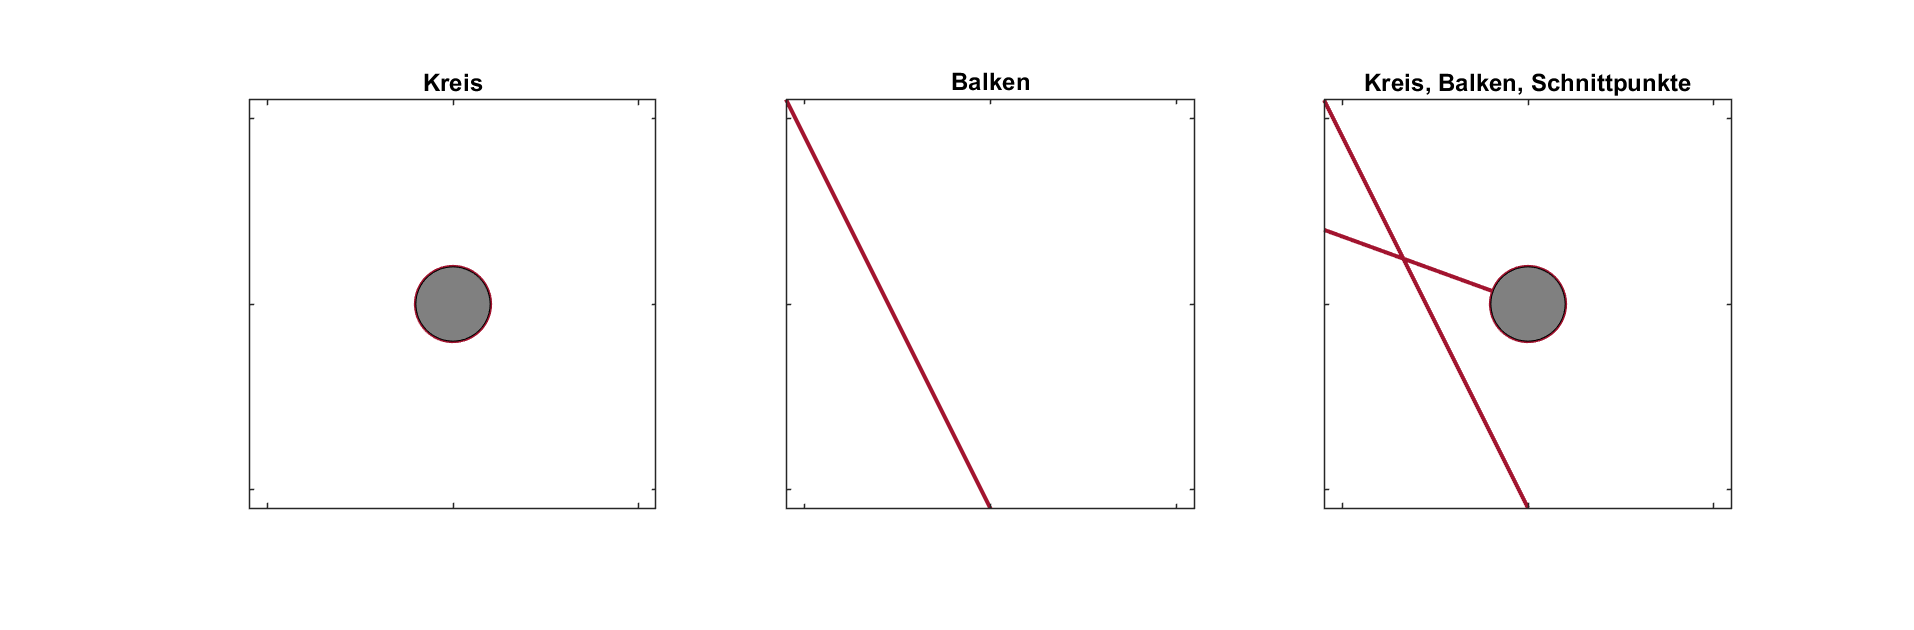
\includegraphics{img/Einheitskreis_Gestalt.png}
\caption{Komponenten eines Netzwerks. Erstellt von ÉD.}
\end{figure}

    R ist so aufgebaut, dass verschiedene Bibliotheken für unterschiedliche
Funktionen geladen werden können. Für die Netzwerkanalyse werden wir auf
das Paket \texttt{igraph}\footnote{https://igraph.org/r/} zurückgreifen.
Mit \texttt{library(\textquotesingle{}igraph\textquotesingle{})} laden
wir das Paket.

    \begin{tcolorbox}[breakable, size=fbox, boxrule=1pt, pad at break*=1mm,colback=cellbackground, colframe=cellborder]
\prompt{In}{incolor}{1}{\boxspacing}
\begin{Verbatim}[commandchars=\\\{\}]
\PY{n+nf}{library}\PY{p}{(}\PY{l+s}{\PYZsq{}}\PY{l+s}{igraph\PYZsq{}}\PY{p}{)}
\end{Verbatim}
\end{tcolorbox}

    \begin{Verbatim}[commandchars=\\\{\}]

Attaching package: ‘igraph’

The following objects are masked from ‘package:stats’:

    decompose, spectrum

The following object is masked from ‘package:base’:

    union

    \end{Verbatim}

    Die Datengrundlage steht bereits in Form einer Auflistung zur
Verfügung,\footnote{https://gist.github.com/LukasCBossert/27fafa33e9b16c33e1107914e928c472},
sodass wir die Daten kopieren und in die nächste Zelle einfügen können.

Fangen wir bei der Funktion \texttt{read.table} an. Es gibt drei
Parameter:

\begin{itemize}
\tightlist
\item
  \texttt{header=TRUE} (es gibt eine Kopfzeile)
\item
  \texttt{sep=","} (die Trennung der Werte erfolgt durch ein Komma)
\item
  \texttt{text=""} (die Werte selbst stehen zwischen den
  Anführungszeichen)
\end{itemize}

Diese Werte übergeben wir der selbstgewählten Variable
\texttt{NFDI\_edges} , was mit dem nach links weisenden Pfeilsymbol
erfolgt.

    \begin{tcolorbox}[breakable, size=fbox, boxrule=1pt, pad at break*=1mm,colback=cellbackground, colframe=cellborder]
\prompt{In}{incolor}{2}{\boxspacing}
\begin{Verbatim}[commandchars=\\\{\}]
\PY{n}{NFDI\PYZus{}edges} \PY{o}{\PYZlt{}\PYZhy{}} \PY{n+nf}{read.table}\PY{p}{(}\PY{n}{header}\PY{o}{=}\PY{k+kc}{TRUE}\PY{p}{,}
                         \PY{n}{sep}\PY{o}{=}\PY{l+s}{\PYZdq{}}\PY{l+s}{,\PYZdq{}}\PY{p}{,}
                         \PY{n}{text}\PY{o}{=}\PY{l+s}{\PYZdq{}}
\PY{l+s}{from,to}
\PY{l+s}{BERD@NFDI,KonsortSWD}
\PY{l+s}{BERD@NFDI,MaRDI}
\PY{l+s}{BERD@NFDI,NFDI4Memory}
\PY{l+s}{BERD@NFDI,Text+}
\PY{l+s}{DAPHNE4NFDI,FAIRmat}
\PY{l+s}{DAPHNE4NFDI,NFDI\PYZhy{}MatWerk}
\PY{l+s}{DAPHNE4NFDI,NFDI4Cat}
\PY{l+s}{DAPHNE4NFDI,NFDI4Chem}
\PY{l+s}{DAPHNE4NFDI,NFDI4Health}
\PY{l+s}{DAPHNE4NFDI,NFDI4Ing}
\PY{l+s}{DAPHNE4NFDI,NFDI4Objects}
\PY{l+s}{DAPHNE4NFDI,PUNCH4NFDI}
\PY{l+s}{FAIRmat,DAPHNE4NFDI}
\PY{l+s}{FAIRmat,DataPLANT}
\PY{l+s}{FAIRmat,MaRDI}
\PY{l+s}{FAIRmat,NFDI\PYZhy{}MatWerk}
\PY{l+s}{FAIRmat,NFDI4Cat}
\PY{l+s}{FAIRmat,NFDI4Chem}
\PY{l+s}{FAIRmat,NFDI4DataScience}
\PY{l+s}{FAIRmat,NFDI4Ing}
\PY{l+s}{FAIRmat,NFDIxCS}
\PY{l+s}{FAIRmat,PUNCH4NFDI}
\PY{l+s}{MaRDI,BERD@NFDI}
\PY{l+s}{MaRDI,FAIRmat}
\PY{l+s}{MaRDI,NFDI\PYZhy{}MatWerk}
\PY{l+s}{MaRDI,NFDI\PYZhy{}Neuro}
\PY{l+s}{MaRDI,NFDI4Cat}
\PY{l+s}{MaRDI,NFDI4Chem}
\PY{l+s}{MaRDI,NFDI4Ing}
\PY{l+s}{MaRDI,PUNCH4NFDI}
\PY{l+s}{NFDI\PYZhy{}MatWerk,DAPHNE4NFDI}
\PY{l+s}{NFDI\PYZhy{}MatWerk,DataPLANT}
\PY{l+s}{NFDI\PYZhy{}MatWerk,FAIRmat}
\PY{l+s}{NFDI\PYZhy{}MatWerk,MaRDI}
\PY{l+s}{NFDI\PYZhy{}MatWerk,NFDI4Chem}
\PY{l+s}{NFDI\PYZhy{}MatWerk,NFDI4DataScience}
\PY{l+s}{NFDI\PYZhy{}MatWerk,NFDI4Ing}
\PY{l+s}{NFDI\PYZhy{}MatWerk,NFDIxCS}
\PY{l+s}{NFDI\PYZhy{}Neuro,DataPLANT}
\PY{l+s}{NFDI\PYZhy{}Neuro,GHGA}
\PY{l+s}{NFDI\PYZhy{}Neuro,NFDI4BioDiversity}
\PY{l+s}{NFDI\PYZhy{}Neuro,NFDI4Culture}
\PY{l+s}{NFDI\PYZhy{}Neuro,NFDI4Earth}
\PY{l+s}{NFDI\PYZhy{}Neuro,NFDI4Health}
\PY{l+s}{NFDI\PYZhy{}Neuro,NFDI4Ing}
\PY{l+s}{NFDI\PYZhy{}Neuro,NFDI4Microbiota}
\PY{l+s}{NFDI4Agri,DataPLANT}
\PY{l+s}{NFDI4Agri,KonsortSWD}
\PY{l+s}{NFDI4Agri,NFDI4BioDiversity}
\PY{l+s}{NFDI4Agri,NFDI4Earth}
\PY{l+s}{NFDI4Agri,NFDI4Health}
\PY{l+s}{NFDI4Agri,NFDI4Immuno}
\PY{l+s}{NFDI4Agri,NFDI4Microbiota}
\PY{l+s}{NFDI4DataScience,KonsortSWD}
\PY{l+s}{NFDI4DataScience,MaRDI}
\PY{l+s}{NFDI4DataScience,NFDI\PYZhy{}MatWerk}
\PY{l+s}{NFDI4DataScience,NFDI4BioDiversity}
\PY{l+s}{NFDI4DataScience,NFDI4Cat}
\PY{l+s}{NFDI4DataScience,NFDI4Chem}
\PY{l+s}{NFDI4DataScience,NFDI4Culture}
\PY{l+s}{NFDI4DataScience,NFDI4Health}
\PY{l+s}{NFDI4DataScience,NFDI4Ing}
\PY{l+s}{NFDI4DataScience,NFDI4Microbiota}
\PY{l+s}{NFDI4DataScience,NFDIxCS}
\PY{l+s}{NFDI4Earth,DataPLANT}
\PY{l+s}{NFDI4Earth,GHGA}
\PY{l+s}{NFDI4Earth,KonsortSWD}
\PY{l+s}{NFDI4Earth,NFDI4Agri}
\PY{l+s}{NFDI4Earth,NFDI4BioDiversity}
\PY{l+s}{NFDI4Earth,NFDI4Cat}
\PY{l+s}{NFDI4Earth,NFDI4Chem}
\PY{l+s}{NFDI4Earth,NFDI4Culture}
\PY{l+s}{NFDI4Earth,NFDI4Health}
\PY{l+s}{NFDI4Earth,NFDI4Ing}
\PY{l+s}{NFDI4Earth,NFDI4Objects}
\PY{l+s}{NFDI4Immuno,GHGA}
\PY{l+s}{NFDI4Immuno,NFDI4Agri}
\PY{l+s}{NFDI4Immuno,NFDI4Health}
\PY{l+s}{NFDI4Immuno,NFDI4Microbiota}
\PY{l+s}{NFDI4Memory,BERD@NFDI}
\PY{l+s}{NFDI4Memory,KonsortSWD}
\PY{l+s}{NFDI4Memory,MaRDI}
\PY{l+s}{NFDI4Memory,NFDI4Culture}
\PY{l+s}{NFDI4Memory,NFDI4Objects}
\PY{l+s}{NFDI4Memory,Text+}
\PY{l+s}{NFDI4Microbiota,DataPLANT}
\PY{l+s}{NFDI4Microbiota,GHGA}
\PY{l+s}{NFDI4Microbiota,NFDI4Agri}
\PY{l+s}{NFDI4Microbiota,NFDI4BioDiversity}
\PY{l+s}{NFDI4Microbiota,NFDI4Chem}
\PY{l+s}{NFDI4Microbiota,NFDI4DataScience}
\PY{l+s}{NFDI4Microbiota,NFDI4Health}
\PY{l+s}{NFDI4Microbiota,NFDI4Immuno}
\PY{l+s}{NFDI4Microbiota,NFDI4Ing}
\PY{l+s}{NFDI4Objects,KonsortSWD}
\PY{l+s}{NFDI4Objects,NFDI4Agri}
\PY{l+s}{NFDI4Objects,NFDI4BioDiversity}
\PY{l+s}{NFDI4Objects,NFDI4Culture}
\PY{l+s}{NFDI4Objects,NFDI4Earth}
\PY{l+s}{NFDI4Objects,NFDI4Memory}
\PY{l+s}{NFDI4Objects,Text+}
\PY{l+s}{NFDI4SD,NFDI4Culture}
\PY{l+s}{NFDI4SD,NFDI4DataScience}
\PY{l+s}{NFDI4SD,NFDI4Memory}
\PY{l+s}{NFDI4SD,NFDI4Objects}
\PY{l+s}{NFDIxCS,FAIRmat}
\PY{l+s}{NFDIxCS,MaRDI}
\PY{l+s}{NFDIxCS,NFDI4Chem}
\PY{l+s}{NFDIxCS,NFDI4DataScience}
\PY{l+s}{NFDIxCS,NFDI4Earth}
\PY{l+s}{NFDIxCS,NFDI4Ing}
\PY{l+s}{PUNCH4NFDI,DAPHNE4NFDI}
\PY{l+s}{PUNCH4NFDI,FAIRmat}
\PY{l+s}{PUNCH4NFDI,GHGA}
\PY{l+s}{PUNCH4NFDI,MaRDI}
\PY{l+s}{PUNCH4NFDI,NFDI4Earth}
\PY{l+s}{PUNCH4NFDI,NFDI4Ing}
\PY{l+s}{PUNCH4NFDI,NFDIxCS}
\PY{l+s}{Text+,KonsortSWD}
\PY{l+s}{Text+,NFDI4BioDiversity}
\PY{l+s}{Text+,NFDI4Culture}
\PY{l+s}{Text+,NFDI4Earth}
\PY{l+s}{Text+,NFDI4Ing}
\PY{l+s}{Text+,NFDI4Memory}
\PY{l+s}{Text+,NFDI4Objects}
\PY{l+s}{\PYZdq{}}\PY{p}{)}
\end{Verbatim}
\end{tcolorbox}

    Damit wir aus diesem Datensatz ein Netzwerk erstellen können, müssen wir
es aufbereiten und einen \texttt{igraph\ graph} erstellen.\footnote{https://igraph.org/r/doc/graph\_from\_data\_frame.html}
Das geschieht mit der Funktion \texttt{graph\_from\_data\_frame}, der
wir unseren Datensatz übergeben.

Zudem geben wir an, dass unser Datensatz bzw. das Netzwerk ungerichtet
ist (\texttt{directed=FALSE}), das heißt, dass die Richtung, wie sie bei
\texttt{from,to} im Datensatz angegeben ist, egal ist. Es geht uns jetzt
nur darum, dass zwei Konsortien verknüpft sind.

    \begin{tcolorbox}[breakable, size=fbox, boxrule=1pt, pad at break*=1mm,colback=cellbackground, colframe=cellborder]
\prompt{In}{incolor}{3}{\boxspacing}
\begin{Verbatim}[commandchars=\\\{\}]
\PY{n}{NFDI\PYZus{}network} \PY{o}{\PYZlt{}\PYZhy{}} \PY{n+nf}{graph\PYZus{}from\PYZus{}data\PYZus{}frame}\PY{p}{(}\PY{n}{NFDI\PYZus{}edges}\PY{p}{,}
                                      \PY{n}{directed}\PY{o}{=}\PY{k+kc}{FALSE}
                                     \PY{p}{)}
\end{Verbatim}
\end{tcolorbox}

    \hypertarget{erstes-netzwerk-grundeinstellung}{%
\subsection{Erstes Netzwerk
(Grundeinstellung)}\label{erstes-netzwerk-grundeinstellung}}

    Zunächst werden wir einen Parameter festlegen, damit unser Netzwerk bei
gleicher Datengrundlage immer gleich aussieht. Dieser Parameter ist
\texttt{seed}. Wir wählen eine beliebige Zahl, die groß sein darf.

Anschließend kommen wir zum eigentlichen Plot. Dafür rufen wir die
Funktion \texttt{plot} auf und übergeben ihr die Variable unseres
Netzwerkgraphen \texttt{NFDI\_network}. Für einen Titel können wir noch
den Parameter \texttt{main} bestimmen und ebenso können wir angeben, ob
wir mit \texttt{frame=TRUE} einen Rahmen um das Netzwerk haben wollen.

    \begin{tcolorbox}[breakable, size=fbox, boxrule=1pt, pad at break*=1mm,colback=cellbackground, colframe=cellborder]
\prompt{In}{incolor}{4}{\boxspacing}
\begin{Verbatim}[commandchars=\\\{\}]
\PY{n+nf}{set.seed}\PY{p}{(}\PY{l+m}{1234}\PY{p}{)}

\PY{n+nf}{plot}\PY{p}{(}\PY{n}{NFDI\PYZus{}network}\PY{p}{,}                    \PY{c+c1}{\PYZsh{} loading data frame}
     \PY{n}{main}  \PY{o}{=} \PY{l+s}{\PYZdq{}}\PY{l+s}{NFDI\PYZhy{}Netzwerk\PYZdq{}}\PY{p}{,}         \PY{c+c1}{\PYZsh{} adding a title}
     \PY{n}{frame} \PY{o}{=} \PY{k+kc}{TRUE}                     \PY{c+c1}{\PYZsh{} making a frame }
     \PY{p}{)}
\end{Verbatim}
\end{tcolorbox}

    \begin{center}
    \adjustimage{max size={0.9\linewidth}{0.9\paperheight}}{das-versprechen-der-vernetzung_files/das-versprechen-der-vernetzung_10_0.png}
    \end{center}
    { \hspace*{\fill} \\}
    
    Wir sehen das Netzwerk der NFDI-Konsortien ohne weitere explizite
Einstellungen.

    \hypertarget{layout-einstellungen}{%
\subsection{Layout-Einstellungen}\label{layout-einstellungen}}

Als nächsten Schritt möchten wir das Layout des Netzwerks optimieren.
Anstatt den Code für den Plot nochmals abzutippen, werden wir den Inhalt
der letzten Zelle markieren, kopieren und in die nächste Zelle einfügen.

Wir erweitern auf diese Weise den Code und arbeiten Schritt für Schritt
am Netzwerk.

Für das Layout von Netzwerken gibt es verschiedene Algorithmen. Je nach
Datensatz kann mal das eine Layout, mal das andere besser geeignet sein.
Mit dem Layout \texttt{graphopt}\footnote{https://igraph.org/r/doc/layout\_with\_graphopt.html}
erzielt man in der Regel ein gutes Ergebnis.

Diesen Wert \texttt{layout.graphopt} übergeben wir dem Parameter
\texttt{layout}.

    \begin{tcolorbox}[breakable, size=fbox, boxrule=1pt, pad at break*=1mm,colback=cellbackground, colframe=cellborder]
\prompt{In}{incolor}{5}{\boxspacing}
\begin{Verbatim}[commandchars=\\\{\}]
\PY{n+nf}{set.seed}\PY{p}{(}\PY{l+m}{1234}\PY{p}{)}

\PY{n+nf}{plot}\PY{p}{(}\PY{n}{NFDI\PYZus{}network}\PY{p}{,}                     \PY{c+c1}{\PYZsh{} loading data frame}
     \PY{n}{main}   \PY{o}{=} \PY{l+s}{\PYZdq{}}\PY{l+s}{NFDI\PYZhy{}Netzwerk\PYZdq{}}\PY{p}{,}         \PY{c+c1}{\PYZsh{} adding a title}
     \PY{n}{frame}  \PY{o}{=} \PY{k+kc}{TRUE}\PY{p}{,}                    \PY{c+c1}{\PYZsh{} making a frame}
     \PY{n}{layout} \PY{o}{=} \PY{n}{layout.graphopt}\PY{p}{,}         \PY{c+c1}{\PYZsh{}* better layout options}
     \PY{p}{)}
\end{Verbatim}
\end{tcolorbox}

    \begin{center}
    \adjustimage{max size={0.9\linewidth}{0.9\paperheight}}{das-versprechen-der-vernetzung_files/das-versprechen-der-vernetzung_13_0.png}
    \end{center}
    { \hspace*{\fill} \\}
    
    Das Netzwerk ist jetzt schon besser strukturiert und die Abstände der
Knoten sind harmonischer.

Wer möchte, der kann weitere Layout-Einstellungen\footnote{https://igraph.org/python/doc/tutorial/tutorial.html\#layout-algorithms}
ausprobieren:

\begin{itemize}
\tightlist
\item
  \texttt{layout\_circle} (\texttt{circle,circular}): Deterministic
  layout that places the vertices on a circle
\item
  \texttt{layout\_drl} (\texttt{drl}): The Distributed Recursive Layout
  algorithm for large graphs
\item
  \texttt{layout\_fruchterman\_reingold} (\texttt{fr}):
  Fruchterman-Reingold force-directed algorithm
\item
  \texttt{layout\_fruchterman\_reingold\_3d} (\texttt{fr3d,\ fr\_3d}):
  Fruchterman-Reingold force-directed algorithm in three dimensions
\item
  \texttt{layout\_grid\_fruchterman\_reingold} (\texttt{grid\_fr}):
  Fruchterman-Reingold force-directed algorithm with grid heuristics for
  large graphs
\item
  \texttt{layout\_kamada\_kawai} (\texttt{kk}): Kamada-Kawai
  force-directed algorithm
\item
  \texttt{layout\_kamada\_kawai\_3d} (\texttt{kk3d,\ kk\_3d}):
  Kamada-Kawai force-directed algorithm in three dimensions
\item
  \texttt{layout\_lgl} (\texttt{large,\ lgl,\ large\_graph}): The Large
  Graph Layout algorithm for large graphs
\item
  \texttt{layout\_random} (\texttt{random}): Places the vertices
  completely randomly
\item
  \texttt{layout\_random\_3d} (\texttt{random\_3d}): Places the vertices
  completely randomly in 3D
\item
  \texttt{layout\_reingold\_tilford} (\texttt{rt,\ tree}):
  Reingold-Tilford tree layout, useful for (almost) tree-like graphs
\item
  \texttt{layout\_reingold\_tilford\_circular}
  (\texttt{rt\_circular,\ tree}): Reingold-Tilford tree layout with a
  polar coordinate post-transformation, useful for (almost) tree-like
  graphs
\item
  \texttt{layout\_sphere} (\texttt{sphere,spherical,circular\_3d}):
  Deterministic layout that places the vertices evenly on the surface of
  a sphere
\end{itemize}

    \hypertarget{farbe-gruxf6uxdfe-kruxfcmmung-knoten-und-kanten}{%
\subsection{Farbe, Größe, Krümmung (Knoten und
Kanten)}\label{farbe-gruxf6uxdfe-kruxfcmmung-knoten-und-kanten}}

Nachdem wir die Anordnung der Knoten optimiert haben, wollen wir im
nächsten Schritt die Darstellung der Knoten und Kanten angehen.

Es lassen sich verschiedene Parameter nach eigenen Wünschen anpassen.

Zunächst möchten wir die Farbe der Knoten angehen. Der Parameter lautet
\texttt{vertex.color} und wir können einen HTML-Farbwert angeben (bspw.
\texttt{\#ffcc66}).\footnote{https://www.w3schools.com/colors/colors\_picker.asp}
Für die Umrandung der Knoten wählen wir den gleichen Farbcode. Der
Parameter lautet \texttt{vertex.frame.color}.

Die Beschriftung der Knoten lässt sich ebenfalls modifizieren. Die
Änderung der Schriftgröße erfolgt über den Parameter
\texttt{vertex.label.cex}, an den wir den Wert \texttt{0.5} übergeben.
Wichtig ist hier, dass der Wert \emph{nicht} in Anführungszeichen
geschrieben wird. Dies ist eine relative Größe und wir möchten die Label
nur halb so groß wie im vorherigen Netzwerk dargestellt haben. Auch die
Farbe der Beschriftung ist änderbar. Ganz analog heißt der Parameter
\texttt{vertex.label.color}, an den wir den Farbwert auch als String,
wie bspw. \texttt{"black"}, übergeben können.

Ein Netzwerk besteht neben den Knoten auch aus Kanten, die zwei Knoten
verbinden. Für die Farbänderung brauchen wir den Parameter
\texttt{edge.color}, an den wir bspw. \texttt{"\#808080"} übergeben.
Neben der Farbe können wir auch den Grad der ``Krümmung'' bestimmen, die
mit \texttt{edge.curved} und dem Wert \texttt{0.1} eingestellt wird.
Wichtig ist auch hier wieder, dass \emph{keine} Anführungszeichen
gesetzt werden.

    \begin{tcolorbox}[breakable, size=fbox, boxrule=1pt, pad at break*=1mm,colback=cellbackground, colframe=cellborder]
\prompt{In}{incolor}{6}{\boxspacing}
\begin{Verbatim}[commandchars=\\\{\}]
\PY{n+nf}{set.seed}\PY{p}{(}\PY{l+m}{1234}\PY{p}{)}


\PY{n+nf}{plot}\PY{p}{(}\PY{n}{NFDI\PYZus{}network}\PY{p}{,}                     \PY{c+c1}{\PYZsh{} loading data frame}
     \PY{n}{main}   \PY{o}{=} \PY{l+s}{\PYZdq{}}\PY{l+s}{NFDI\PYZhy{}Netzwerk\PYZdq{}}\PY{p}{,}         \PY{c+c1}{\PYZsh{} adding a title}
     \PY{n}{frame}  \PY{o}{=} \PY{k+kc}{TRUE}\PY{p}{,}                    \PY{c+c1}{\PYZsh{} making a frame }
     \PY{n}{layout} \PY{o}{=} \PY{n}{layout.graphopt}\PY{p}{,}         \PY{c+c1}{\PYZsh{} better layout options}
     \PY{n}{vertex.color}       \PY{o}{=} \PY{l+s}{\PYZdq{}}\PY{l+s}{\PYZsh{}ffcc66\PYZdq{}}\PY{p}{,}   \PY{c+c1}{\PYZsh{}* color of nodes}
     \PY{n}{vertex.frame.color} \PY{o}{=} \PY{l+s}{\PYZdq{}}\PY{l+s}{\PYZsh{}ffcc66\PYZdq{}}\PY{p}{,}   \PY{c+c1}{\PYZsh{}* color of the frame of nodes}
     \PY{n}{vertex.label.cex}   \PY{o}{=} \PY{l+m}{0.5}\PY{p}{,}         \PY{c+c1}{\PYZsh{}* size of the description of the labels}
     \PY{n}{vertex.label.color} \PY{o}{=} \PY{l+s}{\PYZdq{}}\PY{l+s}{black\PYZdq{}}\PY{p}{,}     \PY{c+c1}{\PYZsh{}* color of the description }
     \PY{n}{edge.color}         \PY{o}{=} \PY{l+s}{\PYZdq{}}\PY{l+s}{\PYZsh{}808080\PYZdq{}}\PY{p}{,}   \PY{c+c1}{\PYZsh{}* color of edges}
     \PY{n}{edge.curved}        \PY{o}{=} \PY{l+m}{0.1}\PY{p}{,}         \PY{c+c1}{\PYZsh{}* factor of \PYZdq{}curvity\PYZdq{}}
     \PY{p}{)}
\end{Verbatim}
\end{tcolorbox}

    \begin{center}
    \adjustimage{max size={0.9\linewidth}{0.9\paperheight}}{das-versprechen-der-vernetzung_files/das-versprechen-der-vernetzung_16_0.png}
    \end{center}
    { \hspace*{\fill} \\}
    
    \hypertarget{knotengruxf6uxdfe-in-abhuxe4ngigkeit-der-kantenanzahl}{%
\subsection{Knotengröße in Abhängigkeit der
Kantenanzahl}\label{knotengruxf6uxdfe-in-abhuxe4ngigkeit-der-kantenanzahl}}

In den bisherigen Netzwerkdarstellungen sind alle Knoten gleich groß.

Jetzt möchten wir eine weitere Informationsebene einbauen und die
Knotengröße entsprechend der Anzahl ihrer Kanten ausgeben.

Die Anzahl der Kanten pro Knoten können wir mit der Funktion
\texttt{degree}\footnote{https://igraph.org/r/doc/degree.html}
ermitteln. Wenn wir dieser Funktion den Datensatz des Netzwerkes
übergeben (\texttt{degree(NFDI\_network)}), dann erhalten wir die Anzahl
der Kanten pro Knoten. Diese Werte nehmen wir als Größeangabe für die
Knoten.

Wir erweitern somit den bisherigen Code um eine Zeile. Die Knotengröße
verbirgt sich hinter dem Parameter \texttt{vertex.size} und als Wert
übergeben wir die Funktion \texttt{degree(NFDI\_network)}.

    \begin{tcolorbox}[breakable, size=fbox, boxrule=1pt, pad at break*=1mm,colback=cellbackground, colframe=cellborder]
\prompt{In}{incolor}{7}{\boxspacing}
\begin{Verbatim}[commandchars=\\\{\}]
\PY{n+nf}{set.seed}\PY{p}{(}\PY{l+m}{1234}\PY{p}{)}

\PY{n+nf}{degree}\PY{p}{(}\PY{n}{NFDI\PYZus{}network}\PY{p}{)}                   \PY{c+c1}{\PYZsh{}* calculate number of edges}

\PY{n+nf}{plot}\PY{p}{(}\PY{n}{NFDI\PYZus{}network}\PY{p}{,}                     \PY{c+c1}{\PYZsh{} loading data frame}
     \PY{n}{main}   \PY{o}{=} \PY{l+s}{\PYZdq{}}\PY{l+s}{NFDI\PYZhy{}Netzwerk\PYZdq{}}\PY{p}{,}         \PY{c+c1}{\PYZsh{} adding a title}
     \PY{n}{frame}  \PY{o}{=} \PY{k+kc}{TRUE}\PY{p}{,}                    \PY{c+c1}{\PYZsh{} making a frame }
     \PY{n}{layout} \PY{o}{=} \PY{n}{layout.graphopt}\PY{p}{,}         \PY{c+c1}{\PYZsh{} better layout options}
     \PY{n}{vertex.color}       \PY{o}{=} \PY{l+s}{\PYZdq{}}\PY{l+s}{\PYZsh{}ffcc66\PYZdq{}}\PY{p}{,}   \PY{c+c1}{\PYZsh{} color of nodes}
     \PY{n}{vertex.frame.color} \PY{o}{=} \PY{l+s}{\PYZdq{}}\PY{l+s}{\PYZsh{}ffcc66\PYZdq{}}\PY{p}{,}   \PY{c+c1}{\PYZsh{} color of the frame of nodes}
     \PY{n}{vertex.label.cex}   \PY{o}{=} \PY{l+m}{0.5}\PY{p}{,}         \PY{c+c1}{\PYZsh{} size of the description of the labels}
     \PY{n}{vertex.label.color} \PY{o}{=} \PY{l+s}{\PYZdq{}}\PY{l+s}{black\PYZdq{}}\PY{p}{,}     \PY{c+c1}{\PYZsh{} color of the description }
                                       \PY{c+c1}{\PYZsh{} color: https://www.w3schools.com/colors/colors\PYZus{}picker.asp }
     \PY{n}{edge.color}         \PY{o}{=} \PY{l+s}{\PYZdq{}}\PY{l+s}{\PYZsh{}808080\PYZdq{}}\PY{p}{,}   \PY{c+c1}{\PYZsh{} color of edges}
     \PY{n}{edge.curved}        \PY{o}{=} \PY{l+m}{0.1}\PY{p}{,}         \PY{c+c1}{\PYZsh{} factor of \PYZdq{}curvity\PYZdq{}}
     \PY{n}{vertex.size}        \PY{o}{=} \PY{n+nf}{degree}\PY{p}{(}\PY{n}{NFDI\PYZus{}network}\PY{p}{)}\PY{p}{,} \PY{c+c1}{\PYZsh{}* size of nodes depends on amount of edges}
     \PY{p}{)}
\end{Verbatim}
\end{tcolorbox}

    \begin{description*}
\item[BERD@NFDI] 6
\item[DAPHNE4NFDI] 11
\item[FAIRmat] 15
\item[MaRDI] 15
\item[NFDI-MatWerk] 12
\item[NFDI-Neuro] 9
\item[NFDI4Agri] 11
\item[NFDI4DataScience] 16
\item[NFDI4Earth] 17
\item[NFDI4Immuno] 6
\item[NFDI4Memory] 10
\item[NFDI4Microbiota] 13
\item[NFDI4Objects] 12
\item[NFDI4SD] 4
\item[NFDIxCS] 10
\item[PUNCH4NFDI] 10
\item[Text+] 10
\item[KonsortSWD] 7
\item[NFDI4Cat] 5
\item[NFDI4Chem] 8
\item[NFDI4Health] 7
\item[NFDI4Ing] 11
\item[DataPLANT] 6
\item[GHGA] 5
\item[NFDI4BioDiversity] 7
\item[NFDI4Culture] 7
\end{description*}


    
    \begin{center}
    \adjustimage{max size={0.9\linewidth}{0.9\paperheight}}{das-versprechen-der-vernetzung_files/das-versprechen-der-vernetzung_18_1.png}
    \end{center}
    { \hspace*{\fill} \\}
    
    \hypertarget{knotengruxf6uxdfe-in-abhuxe4ngigkeit-der-anzahl-ein--und-ausgehender-kanten}{%
\subsection{Knotengröße in Abhängigkeit der Anzahl ein- und ausgehender
Kanten}\label{knotengruxf6uxdfe-in-abhuxe4ngigkeit-der-anzahl-ein--und-ausgehender-kanten}}

Wir haben jetzt eine zweite Informationsebene in unser Netzwerk
eingeführt und können die Knotengröße in Relation zur Kantenanzahl
darstellen.

Im nächsten Schritt möchten wir eine weitere Komponente einführen.
Bislang war es unerheblich, ob ein Konsortium im Datensatz an erster
oder zweiter Stelle genannt wurde, das heißt, es war unerheblich, ob der
aktive oder der passive Kooperationspartner ist.

Jetzt möchten wir die Unterscheidung im Netzwerk berücksichtigen. Dafür
muss unser Graph (Netzwerk) ``gerichtet'' werden\footnote{https://de.wikipedia.org/wiki/Gerichteter\_Graph}.

Wir führen eine neue Variable (\texttt{NFDI\_network\_directed}) ein,
die den Datensatz als gerichteten Graph enthält, was wir mit
\texttt{directed\ =\ TRUE} einstellen.

    \begin{tcolorbox}[breakable, size=fbox, boxrule=1pt, pad at break*=1mm,colback=cellbackground, colframe=cellborder]
\prompt{In}{incolor}{8}{\boxspacing}
\begin{Verbatim}[commandchars=\\\{\}]
\PY{n}{NFDI\PYZus{}network\PYZus{}directed} \PY{o}{\PYZlt{}\PYZhy{}} \PY{n+nf}{graph\PYZus{}from\PYZus{}data\PYZus{}frame}\PY{p}{(}\PY{n}{NFDI\PYZus{}edges}\PY{p}{,}
                                          \PY{n}{directed} \PY{o}{=} \PY{k+kc}{TRUE}
                                         \PY{p}{)}
\end{Verbatim}
\end{tcolorbox}

    Die restlichen Plotangaben übertragen wir aus der vorherigen Zelle.
Entscheidend ist nun, dass wir der Plot-Funktion die neue Variable mit
dem gerichteten Graphen übergeben. Zudem übergeben wir auch der Funktion
\texttt{degree} die neue Variable.

Im gerichteten Netzwerk erschwert die Krümmung der Kanten die
Lesbarkeit. Daher wählen wir für \texttt{edge.curved} den Wert
\texttt{0}.

Ebenso sollen die Pfeilspitzen kleiner werden, was mit
\texttt{edge.arrow.size} und dem relativen Wert \texttt{0.5} möglich
ist.

    \begin{tcolorbox}[breakable, size=fbox, boxrule=1pt, pad at break*=1mm,colback=cellbackground, colframe=cellborder]
\prompt{In}{incolor}{9}{\boxspacing}
\begin{Verbatim}[commandchars=\\\{\}]
\PY{n+nf}{set.seed}\PY{p}{(}\PY{l+m}{1234}\PY{p}{)}

\PY{n+nf}{plot}\PY{p}{(}\PY{n}{NFDI\PYZus{}network\PYZus{}directed}\PY{p}{,}            \PY{c+c1}{\PYZsh{}\PYZlt{}\PYZlt{}\PYZlt{}\PYZlt{}\PYZlt{}\PYZlt{}\PYZlt{} loading data frame}
     \PY{n}{main}   \PY{o}{=} \PY{l+s}{\PYZdq{}}\PY{l+s}{NFDI\PYZhy{}Netzwerk\PYZdq{}}\PY{p}{,}         \PY{c+c1}{\PYZsh{} adding a title}
     \PY{n}{frame}  \PY{o}{=} \PY{k+kc}{TRUE}\PY{p}{,}                    \PY{c+c1}{\PYZsh{} making a frame }
     \PY{n}{layout} \PY{o}{=} \PY{n}{layout.graphopt}\PY{p}{,}         \PY{c+c1}{\PYZsh{} better layout options}
     \PY{n}{vertex.color}       \PY{o}{=} \PY{l+s}{\PYZdq{}}\PY{l+s}{\PYZsh{}ffcc66\PYZdq{}}\PY{p}{,}   \PY{c+c1}{\PYZsh{} color of nodes}
     \PY{n}{vertex.frame.color} \PY{o}{=} \PY{l+s}{\PYZdq{}}\PY{l+s}{\PYZsh{}ffcc66\PYZdq{}}\PY{p}{,}   \PY{c+c1}{\PYZsh{} color of the frame of nodes}
     \PY{n}{vertex.label.cex}   \PY{o}{=} \PY{l+m}{0.5}\PY{p}{,}         \PY{c+c1}{\PYZsh{} size of the description of the labels}
     \PY{n}{vertex.label.color} \PY{o}{=} \PY{l+s}{\PYZdq{}}\PY{l+s}{black\PYZdq{}}\PY{p}{,}     \PY{c+c1}{\PYZsh{} color of the description }
                                       \PY{c+c1}{\PYZsh{} color: https://www.w3schools.com/colors/colors\PYZus{}picker.asp }
     \PY{n}{edge.color}         \PY{o}{=} \PY{l+s}{\PYZdq{}}\PY{l+s}{\PYZsh{}808080\PYZdq{}}\PY{p}{,}   \PY{c+c1}{\PYZsh{} color of edges}
     \PY{n}{edge.curved}        \PY{o}{=} \PY{l+m}{0}\PY{p}{,}           \PY{c+c1}{\PYZsh{}\PYZlt{}\PYZlt{}\PYZlt{}\PYZlt{}\PYZlt{}\PYZlt{}\PYZlt{}\PYZlt{}\PYZlt{} factor of \PYZdq{}curvity\PYZdq{}}
     \PY{n}{vertex.size}        \PY{o}{=} \PY{n+nf}{degree}\PY{p}{(}\PY{n}{NFDI\PYZus{}network\PYZus{}directed}\PY{p}{)}\PY{p}{,} \PY{c+c1}{\PYZsh{}\PYZlt{}\PYZlt{}\PYZlt{}\PYZlt{}\PYZlt{}\PYZlt{} size of nodes depends on amount of edges}
     \PY{n}{edge.arrow.size}    \PY{o}{=} \PY{n}{.}\PY{l+m}{5}\PY{p}{,}          \PY{c+c1}{\PYZsh{}* arrow size,  defaults to 1}
    \PY{p}{)}
\end{Verbatim}
\end{tcolorbox}

    \begin{center}
    \adjustimage{max size={0.9\linewidth}{0.9\paperheight}}{das-versprechen-der-vernetzung_files/das-versprechen-der-vernetzung_22_0.png}
    \end{center}
    { \hspace*{\fill} \\}
    
    Im nächsten Schritt möchten wir die Knotengröße entsprechend der
\emph{ein}gehenden Kanten skalieren. Je öfter ein Konsortium als
Kooperationspartner genannt wird, desto größer wird dessen Knoten.

Wir können dafür die Funktion \texttt{degree} modifizieren, indem wir
\texttt{mode\ =\ "in"} ergänzen\footnote{https://igraph.org/r/doc/degree.html}.

\begin{verbatim}
degree(NFDI_network_directed,
       mode = "in")
\end{verbatim}

    \begin{tcolorbox}[breakable, size=fbox, boxrule=1pt, pad at break*=1mm,colback=cellbackground, colframe=cellborder]
\prompt{In}{incolor}{10}{\boxspacing}
\begin{Verbatim}[commandchars=\\\{\}]
\PY{n+nf}{set.seed}\PY{p}{(}\PY{l+m}{1234}\PY{p}{)}

\PY{n+nf}{degree}\PY{p}{(}\PY{n}{NFDI\PYZus{}network\PYZus{}directed}\PY{p}{,}
       \PY{n}{mode} \PY{o}{=} \PY{l+s}{\PYZdq{}}\PY{l+s}{in\PYZdq{}}\PY{p}{)}


\PY{n+nf}{plot}\PY{p}{(}\PY{n}{NFDI\PYZus{}network\PYZus{}directed}\PY{p}{,}            \PY{c+c1}{\PYZsh{} loading data frame}
     \PY{n}{main}   \PY{o}{=} \PY{l+s}{\PYZdq{}}\PY{l+s}{NFDI\PYZhy{}Netzwerk (\PYZlt{}in\PYZgt{})\PYZdq{}}\PY{p}{,}  \PY{c+c1}{\PYZsh{}\PYZlt{}\PYZlt{}\PYZlt{}\PYZlt{}\PYZlt{}\PYZlt{}\PYZlt{}\PYZlt{} adding a title}
     \PY{n}{frame}  \PY{o}{=} \PY{k+kc}{TRUE}\PY{p}{,}                    \PY{c+c1}{\PYZsh{} making a frame }
     \PY{n}{layout} \PY{o}{=} \PY{n}{layout.graphopt}\PY{p}{,}         \PY{c+c1}{\PYZsh{} better layout options}
     \PY{n}{vertex.color}       \PY{o}{=} \PY{l+s}{\PYZdq{}}\PY{l+s}{\PYZsh{}ffcc66\PYZdq{}}\PY{p}{,}   \PY{c+c1}{\PYZsh{} color of nodes}
     \PY{n}{vertex.frame.color} \PY{o}{=} \PY{l+s}{\PYZdq{}}\PY{l+s}{\PYZsh{}ffcc66\PYZdq{}}\PY{p}{,}   \PY{c+c1}{\PYZsh{} color of the frame of nodes}
     \PY{n}{vertex.label.cex}   \PY{o}{=} \PY{l+m}{0.5}\PY{p}{,}         \PY{c+c1}{\PYZsh{} size of the description of the labels}
     \PY{n}{vertex.label.color} \PY{o}{=} \PY{l+s}{\PYZdq{}}\PY{l+s}{black\PYZdq{}}\PY{p}{,}     \PY{c+c1}{\PYZsh{} color of the description }
                                       \PY{c+c1}{\PYZsh{} color: https://www.w3schools.com/colors/colors\PYZus{}picker.asp }
     \PY{n}{edge.color}         \PY{o}{=} \PY{l+s}{\PYZdq{}}\PY{l+s}{\PYZsh{}808080\PYZdq{}}\PY{p}{,}   \PY{c+c1}{\PYZsh{} color of edges}
     \PY{n}{edge.curved}        \PY{o}{=} \PY{l+m}{0}\PY{p}{,}           \PY{c+c1}{\PYZsh{} factor of \PYZdq{}curvity\PYZdq{}}
     \PY{n}{vertex.size}        \PY{o}{=} \PY{n+nf}{degree}\PY{p}{(}\PY{n}{NFDI\PYZus{}network\PYZus{}directed}\PY{p}{,}
                                 \PY{n}{mode} \PY{o}{=} \PY{l+s}{\PYZdq{}}\PY{l+s}{in\PYZdq{}}\PY{p}{)}\PY{p}{,} \PY{c+c1}{\PYZsh{}\PYZlt{}\PYZlt{}\PYZlt{}\PYZlt{}\PYZlt{}\PYZlt{} size of nodes depends on amount of edges}
     \PY{n}{edge.arrow.size}    \PY{o}{=} \PY{n}{.}\PY{l+m}{5}\PY{p}{,}          \PY{c+c1}{\PYZsh{} arrow size,  defaults to 1}
    \PY{p}{)}
\end{Verbatim}
\end{tcolorbox}

    \begin{description*}
\item[BERD@NFDI] 2
\item[DAPHNE4NFDI] 3
\item[FAIRmat] 5
\item[MaRDI] 7
\item[NFDI-MatWerk] 4
\item[NFDI-Neuro] 1
\item[NFDI4Agri] 4
\item[NFDI4DataScience] 5
\item[NFDI4Earth] 6
\item[NFDI4Immuno] 2
\item[NFDI4Memory] 4
\item[NFDI4Microbiota] 4
\item[NFDI4Objects] 5
\item[NFDI4SD] 0
\item[NFDIxCS] 4
\item[PUNCH4NFDI] 3
\item[Text+] 3
\item[KonsortSWD] 7
\item[NFDI4Cat] 5
\item[NFDI4Chem] 8
\item[NFDI4Health] 7
\item[NFDI4Ing] 11
\item[DataPLANT] 6
\item[GHGA] 5
\item[NFDI4BioDiversity] 7
\item[NFDI4Culture] 7
\end{description*}


    
    \begin{center}
    \adjustimage{max size={0.9\linewidth}{0.9\paperheight}}{das-versprechen-der-vernetzung_files/das-versprechen-der-vernetzung_24_1.png}
    \end{center}
    { \hspace*{\fill} \\}
    
    Ebenfalls können wir nun auch die Größe der Konsortien entsprechend
ihrer \emph{aus}gehenden Kanten darstellen.

Wir übernehmen den kompletten Zelleninhalt von zuvor und ändern
lediglich \texttt{in} zu \texttt{out}.

    \begin{tcolorbox}[breakable, size=fbox, boxrule=1pt, pad at break*=1mm,colback=cellbackground, colframe=cellborder]
\prompt{In}{incolor}{11}{\boxspacing}
\begin{Verbatim}[commandchars=\\\{\}]
\PY{n+nf}{set.seed}\PY{p}{(}\PY{l+m}{1234}\PY{p}{)}

\PY{n+nf}{degree}\PY{p}{(}\PY{n}{NFDI\PYZus{}network\PYZus{}directed}\PY{p}{,}
       \PY{n}{mode} \PY{o}{=} \PY{l+s}{\PYZdq{}}\PY{l+s}{out\PYZdq{}}\PY{p}{)}

\PY{n+nf}{plot}\PY{p}{(}\PY{n}{NFDI\PYZus{}network\PYZus{}directed}\PY{p}{,}            \PY{c+c1}{\PYZsh{} loading data frame}
     \PY{n}{main}   \PY{o}{=} \PY{l+s}{\PYZdq{}}\PY{l+s}{NFDI\PYZhy{}Netzwerk (\PYZlt{}out\PYZgt{})\PYZdq{}}\PY{p}{,}  \PY{c+c1}{\PYZsh{}\PYZlt{}\PYZlt{}\PYZlt{}\PYZlt{}\PYZlt{}\PYZlt{}\PYZlt{}\PYZlt{} adding a title}
     \PY{n}{frame}  \PY{o}{=} \PY{k+kc}{TRUE}\PY{p}{,}                    \PY{c+c1}{\PYZsh{} making a frame }
     \PY{n}{layout} \PY{o}{=} \PY{n}{layout.graphopt}\PY{p}{,}         \PY{c+c1}{\PYZsh{} better layout options}
     \PY{n}{vertex.color}       \PY{o}{=} \PY{l+s}{\PYZdq{}}\PY{l+s}{\PYZsh{}ffcc66\PYZdq{}}\PY{p}{,}   \PY{c+c1}{\PYZsh{} color of nodes}
     \PY{n}{vertex.frame.color} \PY{o}{=} \PY{l+s}{\PYZdq{}}\PY{l+s}{\PYZsh{}ffcc66\PYZdq{}}\PY{p}{,}   \PY{c+c1}{\PYZsh{} color of the frame of nodes}
     \PY{n}{vertex.label.cex}   \PY{o}{=} \PY{l+m}{0.5}\PY{p}{,}         \PY{c+c1}{\PYZsh{} size of the description of the labels}
     \PY{n}{vertex.label.color} \PY{o}{=} \PY{l+s}{\PYZdq{}}\PY{l+s}{black\PYZdq{}}\PY{p}{,}     \PY{c+c1}{\PYZsh{} color of the description }
                                       \PY{c+c1}{\PYZsh{} color: https://www.w3schools.com/colors/colors\PYZus{}picker.asp }
     \PY{n}{edge.color}         \PY{o}{=} \PY{l+s}{\PYZdq{}}\PY{l+s}{\PYZsh{}808080\PYZdq{}}\PY{p}{,}   \PY{c+c1}{\PYZsh{} color of edges}
     \PY{n}{edge.curved}        \PY{o}{=} \PY{l+m}{0}\PY{p}{,}           \PY{c+c1}{\PYZsh{} factor of \PYZdq{}curvity\PYZdq{}}
     \PY{n}{vertex.size}        \PY{o}{=} \PY{n+nf}{degree}\PY{p}{(}\PY{n}{NFDI\PYZus{}network\PYZus{}directed}\PY{p}{,}
                                 \PY{n}{mode} \PY{o}{=} \PY{l+s}{\PYZdq{}}\PY{l+s}{out\PYZdq{}}\PY{p}{)}\PY{p}{,} \PY{c+c1}{\PYZsh{}\PYZlt{}\PYZlt{}\PYZlt{}\PYZlt{}\PYZlt{}\PYZlt{} size of nodes depends on amount of edges}
     \PY{n}{edge.arrow.size}    \PY{o}{=} \PY{n}{.}\PY{l+m}{5}\PY{p}{,}          \PY{c+c1}{\PYZsh{} arrow size,  defaults to 1}
    \PY{p}{)}
\end{Verbatim}
\end{tcolorbox}

    \begin{description*}
\item[BERD@NFDI] 4
\item[DAPHNE4NFDI] 8
\item[FAIRmat] 10
\item[MaRDI] 8
\item[NFDI-MatWerk] 8
\item[NFDI-Neuro] 8
\item[NFDI4Agri] 7
\item[NFDI4DataScience] 11
\item[NFDI4Earth] 11
\item[NFDI4Immuno] 4
\item[NFDI4Memory] 6
\item[NFDI4Microbiota] 9
\item[NFDI4Objects] 7
\item[NFDI4SD] 4
\item[NFDIxCS] 6
\item[PUNCH4NFDI] 7
\item[Text+] 7
\item[KonsortSWD] 0
\item[NFDI4Cat] 0
\item[NFDI4Chem] 0
\item[NFDI4Health] 0
\item[NFDI4Ing] 0
\item[DataPLANT] 0
\item[GHGA] 0
\item[NFDI4BioDiversity] 0
\item[NFDI4Culture] 0
\end{description*}


    
    \begin{center}
    \adjustimage{max size={0.9\linewidth}{0.9\paperheight}}{das-versprechen-der-vernetzung_files/das-versprechen-der-vernetzung_26_1.png}
    \end{center}
    { \hspace*{\fill} \\}
    
    Es fällt auf, dass einige Knoten schrumpfen und in der Tabelle sieht
man, dass sie den Wert \texttt{0} bei ausgehenden Kanten haben. Das
liegt daran, dass dies die Konsortien sind, die in der ersten
Förderrunde bereits bewilligt wurden und daher keinen neuen Letters of
Intent eingereicht haben. Unser Datensatz berücksichtigt ja nur die
Letters of Intent der zweiten Förderrunde. Die Konsortien der ersten
Runde können daher nur als ``passive'' Kooperationspartner genannt
werden.

\hypertarget{ausschluss-der-konsortien-aus-der-ersten-fuxf6rderrunde}{%
\subsection{Ausschluss der Konsortien aus der ersten
Förderrunde}\label{ausschluss-der-konsortien-aus-der-ersten-fuxf6rderrunde}}

Wir können nun mal schauen, wie sich das Netzwerk ändert, wenn wir die
bereits geförderten Konsortien ausschließen. Damit bekommen wir ein
Netzwerk, das nur die Kooperationen der Konsortien der zweiten
Förderrunde berücksichtigt.

Der Filter bzw. das Löschen der besagten Konsortien funktioniert so: Die
Funktion \texttt{delete\_vertices} kümmert sich um die Löschung wir
müssen dafür zunächst den Netzwerkgraphen angeben, anschließend findet
eine Berechnung statt: Es sollen alle Knoten/Konsortien (ausgegeben
durch die Funktion \texttt{V}) gelöscht werden, deren Anzahl an Kanten
im Modus \texttt{out} gleich \texttt{0} ist. Diese gelöschte Knoten
übergeben wir der neuen Variable
\texttt{NFDI\_network\_directed\_filter}, die wir weiter nutzen können.

Als Darstellungsmodus des Netzwerks wähle ich \texttt{total}, da es mir
jetzt nicht um die separate Anzahl der ein- und ausgehenden
Verbindungen, sondern um deren Summe geht.

    \begin{tcolorbox}[breakable, size=fbox, boxrule=1pt, pad at break*=1mm,colback=cellbackground, colframe=cellborder]
\prompt{In}{incolor}{12}{\boxspacing}
\begin{Verbatim}[commandchars=\\\{\}]
\PY{n+nf}{set.seed}\PY{p}{(}\PY{l+m}{1234}\PY{p}{)}

\PY{n}{NFDI\PYZus{}network\PYZus{}directed\PYZus{}filter} \PY{o}{\PYZlt{}\PYZhy{}} \PY{n+nf}{delete\PYZus{}vertices}\PY{p}{(}\PY{n}{NFDI\PYZus{}network\PYZus{}directed}\PY{p}{,} 
            \PY{n+nf}{V}\PY{p}{(}\PY{n}{NFDI\PYZus{}network\PYZus{}directed}\PY{p}{)}\PY{p}{[} \PY{n+nf}{degree}\PY{p}{(}\PY{n}{NFDI\PYZus{}network\PYZus{}directed}\PY{p}{,} \PY{n}{mode} \PY{o}{=} \PY{l+s}{\PYZdq{}}\PY{l+s}{out\PYZdq{}}\PY{p}{)} \PY{o}{==} \PY{l+m}{0} \PY{p}{]}\PY{p}{)}

\PY{n+nf}{degree}\PY{p}{(}\PY{n}{NFDI\PYZus{}network\PYZus{}directed\PYZus{}filter}\PY{p}{,}
       \PY{n}{mode} \PY{o}{=} \PY{l+s}{\PYZdq{}}\PY{l+s}{total\PYZdq{}}\PY{p}{)}

\PY{n+nf}{plot}\PY{p}{(}\PY{n}{NFDI\PYZus{}network\PYZus{}directed\PYZus{}filter}\PY{p}{,}           \PY{c+c1}{\PYZsh{}\PYZlt{}\PYZlt{}\PYZlt{}\PYZlt{}\PYZlt{}\PYZlt{}\PYZlt{}\PYZlt{} loading data frame}
     \PY{n}{main}   \PY{o}{=} \PY{l+s}{\PYZdq{}}\PY{l+s}{NFDI\PYZhy{}Netzwerk (\PYZlt{}filtered\PYZgt{})\PYZdq{}}\PY{p}{,}  \PY{c+c1}{\PYZsh{}\PYZlt{}\PYZlt{}\PYZlt{}\PYZlt{}\PYZlt{}\PYZlt{}\PYZlt{}\PYZlt{} adding a title}
     \PY{n}{frame}  \PY{o}{=} \PY{k+kc}{TRUE}\PY{p}{,}                    \PY{c+c1}{\PYZsh{} making a frame }
     \PY{n}{layout} \PY{o}{=} \PY{n}{layout.graphopt}\PY{p}{,}         \PY{c+c1}{\PYZsh{} better layout options}
     \PY{n}{vertex.color}       \PY{o}{=} \PY{l+s}{\PYZdq{}}\PY{l+s}{\PYZsh{}ffcc66\PYZdq{}}\PY{p}{,}   \PY{c+c1}{\PYZsh{} color of nodes}
     \PY{n}{vertex.frame.color} \PY{o}{=} \PY{l+s}{\PYZdq{}}\PY{l+s}{\PYZsh{}ffcc66\PYZdq{}}\PY{p}{,}   \PY{c+c1}{\PYZsh{} color of the frame of nodes}
     \PY{n}{vertex.label.cex}   \PY{o}{=} \PY{l+m}{0.5}\PY{p}{,}         \PY{c+c1}{\PYZsh{} size of the description of the labels}
     \PY{n}{vertex.label.color} \PY{o}{=} \PY{l+s}{\PYZdq{}}\PY{l+s}{black\PYZdq{}}\PY{p}{,}     \PY{c+c1}{\PYZsh{} color of the description }
                                       \PY{c+c1}{\PYZsh{} color: https://www.w3schools.com/colors/colors\PYZus{}picker.asp }
     \PY{n}{edge.color}         \PY{o}{=} \PY{l+s}{\PYZdq{}}\PY{l+s}{\PYZsh{}808080\PYZdq{}}\PY{p}{,}   \PY{c+c1}{\PYZsh{} color of edges}
     \PY{n}{edge.curved}        \PY{o}{=} \PY{l+m}{0}\PY{p}{,}           \PY{c+c1}{\PYZsh{} factor of \PYZdq{}curvity\PYZdq{}}
     \PY{n}{vertex.size}        \PY{o}{=} \PY{n+nf}{degree}\PY{p}{(}\PY{n}{NFDI\PYZus{}network\PYZus{}directed\PYZus{}filter}\PY{p}{,}
                                 \PY{n}{mode} \PY{o}{=} \PY{l+s}{\PYZdq{}}\PY{l+s}{total\PYZdq{}}\PY{p}{)}\PY{p}{,} \PY{c+c1}{\PYZsh{}\PYZlt{}\PYZlt{}\PYZlt{}\PYZlt{}\PYZlt{}\PYZlt{} size of nodes depends on amount of edges}
     \PY{n}{edge.arrow.size}    \PY{o}{=} \PY{n}{.}\PY{l+m}{5}\PY{p}{,}          \PY{c+c1}{\PYZsh{} arrow size,  defaults to 1}
    \PY{p}{)}
\end{Verbatim}
\end{tcolorbox}

    \begin{description*}
\item[BERD@NFDI] 5
\item[DAPHNE4NFDI] 7
\item[FAIRmat] 11
\item[MaRDI] 12
\item[NFDI-MatWerk] 9
\item[NFDI-Neuro] 3
\item[NFDI4Agri] 7
\item[NFDI4DataScience] 9
\item[NFDI4Earth] 8
\item[NFDI4Immuno] 4
\item[NFDI4Memory] 8
\item[NFDI4Microbiota] 7
\item[NFDI4Objects] 9
\item[NFDI4SD] 3
\item[NFDIxCS] 8
\item[PUNCH4NFDI] 8
\item[Text+] 6
\end{description*}


    
    \begin{center}
    \adjustimage{max size={0.9\linewidth}{0.9\paperheight}}{das-versprechen-der-vernetzung_files/das-versprechen-der-vernetzung_28_1.png}
    \end{center}
    { \hspace*{\fill} \\}
    
    \hypertarget{netzwerkanalyse}{%
\section{Netzwerkanalyse}\label{netzwerkanalyse}}

Nach den bisherigen Runden der Netzwerkvisualisierung wollen wir noch
einen Schritt weiter gehen und die Netzwerkstruktur analysieren.

\hypertarget{nfdi-konferenzsystematik}{%
\subsection{NFDI-Konferenzsystematik}\label{nfdi-konferenzsystematik}}

Als ersten Schritt wollen wir die Knoten bzw. Konsortien in den Farben
der NFDI-Konferenzsystematik einfärben.

Wie kommt die NFDI-Konferenzsystematik zustande? Für die Vorträge wurden
fünf Panels aufgemacht:

\begin{enumerate}
\def\labelenumi{\arabic{enumi}.}
\tightlist
\item
  Medizin
\item
  Lebenswissenschaften
\item
  Geisteswissenschaften
\item
  Ingenieurwissenschaften
\item
  Chemie/Physik
\end{enumerate}

Die antragsstellenden Konsortien wurden auf diese fünf Gruppen
eingeteilt:\footnote{https://www.dfg.de/download/pdf/foerderung/programme/nfdi/nfdi\_konferenz\_2020/programm\_webkonferenz\_2020.pdf}

\begin{figure}
\centering
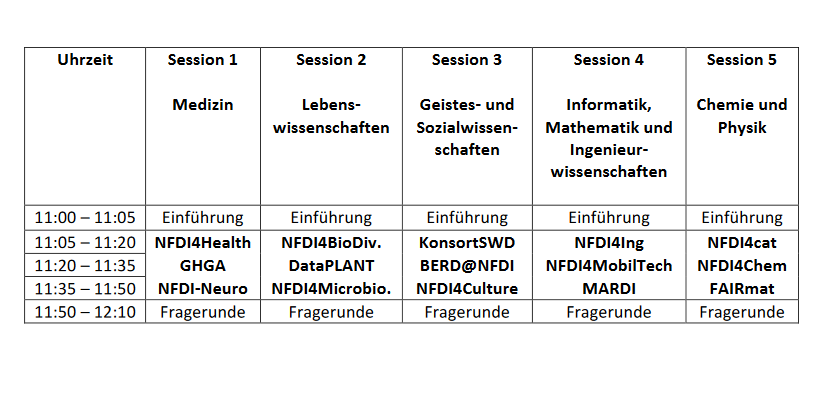
\includegraphics{img/nfdi-konferenzsystematik.png}
\caption{Konferenzsystematik}
\end{figure}

Auffällig ist, dass nach der DFG-Fachsystematik die Naturwissenschaften
auf die Lebenswissenschaften, Ingenieurwissenschaften und Chemie/Physik
aufgeteilt worden sind, wie man im folgenden Sankey (Flussdiagramm)
sehen kann.

\begin{figure}
\centering
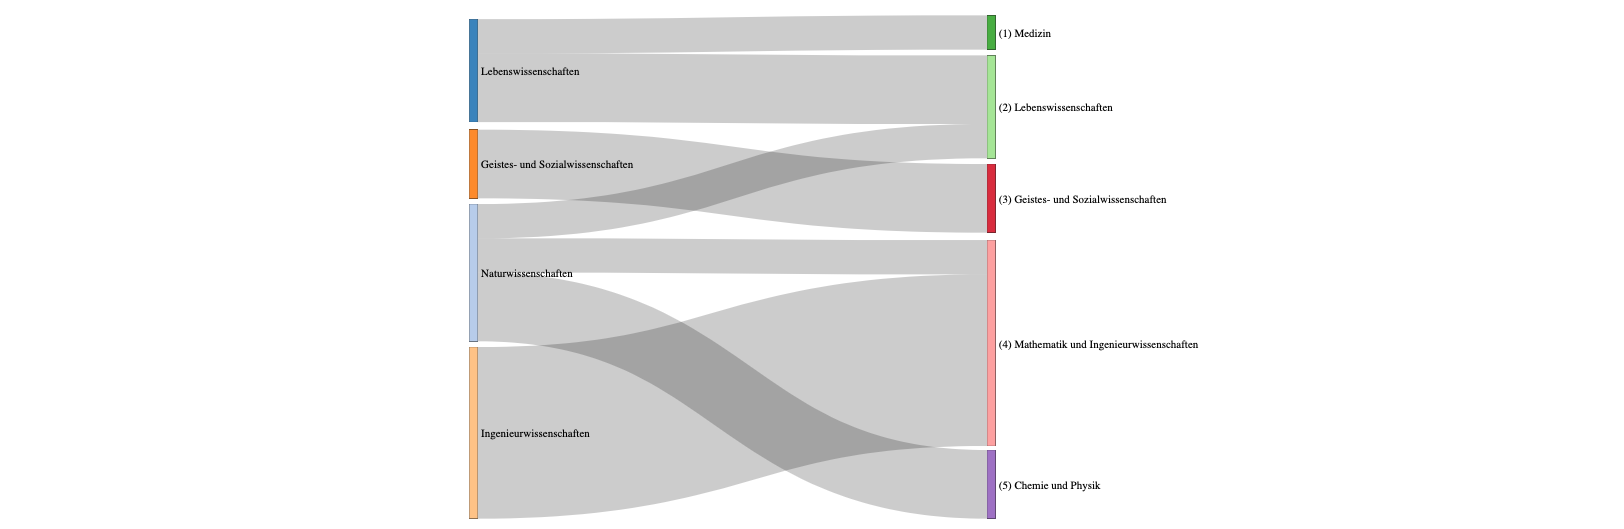
\includegraphics{img/dfg-nfdi-sankey.png}
\caption{Sankey}
\end{figure}

Alle Konsortien sind also einem dieser fünf Bereiche zugeteilt und wir
wollen das nun im Netzwerk zeigen. Diese Einteilung der Konsortien auf
die Konferenzsystematik laden wir in der nächsten Zelle.

Dieser neue Datensatz wird der Variable \texttt{NFDI\_nodes} übergeben;
die erste Spalte beinhaltet die Konsortialnamen, die zweite Spalte die
Nummer aus der NFDI-\emph{Konferenz}systematik.

    \begin{tcolorbox}[breakable, size=fbox, boxrule=1pt, pad at break*=1mm,colback=cellbackground, colframe=cellborder]
\prompt{In}{incolor}{13}{\boxspacing}
\begin{Verbatim}[commandchars=\\\{\}]
\PY{n}{NFDI\PYZus{}nodes} \PY{o}{\PYZlt{}\PYZhy{}} \PY{n+nf}{read.table}\PY{p}{(}\PY{n}{header}\PY{o}{=}\PY{k+kc}{TRUE}\PY{p}{,}
                         \PY{n}{sep}\PY{o}{=}\PY{l+s}{\PYZdq{}}\PY{l+s}{,\PYZdq{}}\PY{p}{,}
                         \PY{n}{text}\PY{o}{=}\PY{l+s}{\PYZdq{}}
\PY{l+s}{name,group}
\PY{l+s}{BERD@NFDI,3}
\PY{l+s}{DAPHNE4NFDI,5}
\PY{l+s}{DataPLANT,2}
\PY{l+s}{FAIRmat,5}
\PY{l+s}{GHGA,1}
\PY{l+s}{KonsortSWD,3}
\PY{l+s}{MaRDI,4}
\PY{l+s}{NFDI\PYZhy{}MatWerk,4}
\PY{l+s}{NFDI\PYZhy{}Neuro,1}
\PY{l+s}{NFDI4Agri,2}
\PY{l+s}{NFDI4BioDiversity,2}
\PY{l+s}{NFDI4Cat,5}
\PY{l+s}{NFDI4Chem,5}
\PY{l+s}{NFDI4Culture,3}
\PY{l+s}{NFDI4DataScience,4}
\PY{l+s}{NFDI4Earth,2}
\PY{l+s}{NFDI4Health,1}
\PY{l+s}{NFDI4Immuno,1}
\PY{l+s}{NFDI4Ing,4}
\PY{l+s}{NFDI4Memory,3}
\PY{l+s}{NFDI4Microbiota,2}
\PY{l+s}{NFDI4Objects,3}
\PY{l+s}{NFDI4SD,3}
\PY{l+s}{NFDIxCS,4}
\PY{l+s}{PUNCH4NFDI,5}
\PY{l+s}{Text+,3}
\PY{l+s}{\PYZdq{}}\PY{p}{)}
\end{Verbatim}
\end{tcolorbox}

    Jetzt müssen wir aus dem Datensatz noch ein Graph-Datensatz erstellen,
was wiederum mit \texttt{graph\_from\_data\_frame} geschieht. Neu ist,
dass wir nun differenzieren, was unser Kanten-Data-Frame und was die
Liste mit den Knoten ist.

    \begin{tcolorbox}[breakable, size=fbox, boxrule=1pt, pad at break*=1mm,colback=cellbackground, colframe=cellborder]
\prompt{In}{incolor}{14}{\boxspacing}
\begin{Verbatim}[commandchars=\\\{\}]
\PY{n}{NFDI\PYZus{}network\PYZus{}directed} \PY{o}{\PYZlt{}\PYZhy{}} \PY{n+nf}{graph\PYZus{}from\PYZus{}data\PYZus{}frame}\PY{p}{(}\PY{n}{d} \PY{o}{=} \PY{n}{NFDI\PYZus{}edges}\PY{p}{,}        \PY{c+c1}{\PYZsh{} d = data frame =\PYZti{} edges}
                                               \PY{n}{vertices} \PY{o}{=} \PY{n}{NFDI\PYZus{}nodes}\PY{p}{,} \PY{c+c1}{\PYZsh{}nodes}
                                               \PY{n}{directed} \PY{o}{=} \PY{k+kc}{TRUE}\PY{p}{)}       \PY{c+c1}{\PYZsh{}directed}
\end{Verbatim}
\end{tcolorbox}

    \hypertarget{nfdi-farbkodierung}{%
\subsection{NFDI-Farbkodierung}\label{nfdi-farbkodierung}}

Damit wir die Knoteneinteilung auf die NFDI-Konferenzsystematik im
Netzwerk besser erkennen, wählen wir eine Farbcodierung entsprechend der
DFG-Fachsystematik (ggf. leichte Anpassung).

Es gelten folgende Werte

\begin{longtable}[]{@{}clc@{}}
\toprule
Nr. & Bezeichnung & HTML-Farbcode\tabularnewline
\midrule
\endhead
(1) & Medizin & \texttt{\#f5ac9f}\tabularnewline
(2) & Lebenswissenschaften & \texttt{\#e43516}\tabularnewline
(3) & Geisteswissenschaften & \texttt{\#f9b900}\tabularnewline
(4) & Ingenieurwissenschaften & \texttt{\#007aaf}\tabularnewline
(5) & Chemie/Physik & \texttt{\#6ca11d}\tabularnewline
\bottomrule
\end{longtable}

Diese Farbwerte geben wir jetzt der Reihe nach an die Variable
\texttt{NFDI\_color\_code} weiter, dabei werden die Farbwerte in eine
Liste geschrieben. Anhand der Funktion \texttt{c} werden die Werte in
einen Vektor geschrieben,\footnote{https://www.rdocumentation.org/packages/base/versions/3.6.2/topics/c}
mit dem wir weiterarbeiten können.

Jetzt müssen wir noch die Verknüpfung zwischen Farbwert und den
Konsortien herstellen. Dafür führen wir die Variable
\texttt{NFDI\_color\_groups} ein: Jeder Wert aus
\texttt{NFDI\_color\_code} hat eine Positionsnummer (1-5), das nutzen
wir, indem wir den Wert der zweiten Spalte des Netzwerkgraphen
(\texttt{\$group}) als Zahl auswerten und so den Farbwert übergeben.
Vereinfacht gesagt und vom Ergebnis her gesehen, bekommt die Nummer der
NFDI-Konferenzsystematik den Farbwert, der an der entsprechenden Stelle
in der Liste der Variable \texttt{NFDI\_color\_code} steht.

    \begin{tcolorbox}[breakable, size=fbox, boxrule=1pt, pad at break*=1mm,colback=cellbackground, colframe=cellborder]
\prompt{In}{incolor}{15}{\boxspacing}
\begin{Verbatim}[commandchars=\\\{\}]
\PY{n}{NFDI\PYZus{}color\PYZus{}code} \PY{o}{\PYZlt{}\PYZhy{}} \PY{n+nf}{c}\PY{p}{(}\PY{l+s}{\PYZdq{}}\PY{l+s}{\PYZsh{}f5ac9f\PYZdq{}}\PY{p}{,} \PY{c+c1}{\PYZsh{} Medizin}
                     \PY{l+s}{\PYZdq{}}\PY{l+s}{\PYZsh{}e43516\PYZdq{}}\PY{p}{,} \PY{c+c1}{\PYZsh{} Lebenswissenschaften}
                     \PY{l+s}{\PYZdq{}}\PY{l+s}{\PYZsh{}f9b900\PYZdq{}}\PY{p}{,} \PY{c+c1}{\PYZsh{} Geisteswissenschaften}
                     \PY{l+s}{\PYZdq{}}\PY{l+s}{\PYZsh{}007aaf\PYZdq{}}\PY{p}{,} \PY{c+c1}{\PYZsh{} Ingenieurwissenschaften}
                     \PY{l+s}{\PYZdq{}}\PY{l+s}{\PYZsh{}6ca11d\PYZdq{}}  \PY{c+c1}{\PYZsh{} Chemie/Physik}
                    \PY{p}{)}
\PY{n}{NFDI\PYZus{}color\PYZus{}groups} \PY{o}{\PYZlt{}\PYZhy{}} \PY{n}{NFDI\PYZus{}color\PYZus{}code}\PY{p}{[}\PY{n+nf}{as.numeric}\PY{p}{(}\PY{n+nf}{as.factor}\PY{p}{(}\PY{n+nf}{V}\PY{p}{(}\PY{n}{NFDI\PYZus{}network\PYZus{}directed}\PY{p}{)}\PY{o}{\PYZdl{}}\PY{n}{group}\PY{p}{)}\PY{p}{)}\PY{p}{]}
\end{Verbatim}
\end{tcolorbox}

    \hypertarget{netzwerk-mit-eingefuxe4rbten-knoten}{%
\subsection{Netzwerk mit eingefärbten
Knoten}\label{netzwerk-mit-eingefuxe4rbten-knoten}}

Wir können wiederum den Code der vorhergehenden Zelle übernehmen und
anpassen.

Entscheidend ist, dass wir bei \texttt{vertex.color} und
\texttt{vertex.frame.color} die Variable \texttt{NFDI\_color\_groups}
als Wert angeben. Wir wollen ebenfalls das gesamte Netzwerk mit allen
Kanten (\texttt{mode\ =\ "total"}) berücksichtigen und darstellen.

Was jetzt noch fehlt, ist eine Legende, sodass wir auch sehen, was
hinter der Farbcodierung steckt.

Dafür gibt es eine spezielle Funktion \texttt{legend}, die wir nun mit
Werten füllen.

Zunächst die Positionierung der Legende, die wir ``unten rechts''
(\texttt{"bottomright"}) haben wollen, dann der Titel
(\texttt{title\ =\ "NFDI-Konferenzsystematik"}), jetzt kommt der Inhalt
der Legende, was über den Parameter \texttt{legend} geregelt wird:
Hierfür bauen wir uns wiederum eine Liste (\texttt{c()}), in der wir die
gewünschten Werte eintragen.

Mit \texttt{col} wird das Farbschema festgesetzt und wir können direkt
auf die NFDI-Farbliste über die Variable \texttt{NFDI\_color\_code}
verweisen.

Wir dürfen auf keinen Fall den Parameter \texttt{pch} vergessen, da
hierüber das Symbol in der Legende definiert wird. Mit dem Wert
\texttt{20} wählen wir einen ausgefüllten Kreis.

Mit \texttt{bty} und dem Wert \texttt{n} für \texttt{no} verzichten wir
auf einen Rahmen um die Legende.

\texttt{cex} (also \texttt{character\ expansion}) ist wieder ein
relativer Wert und wir können die Schriftgröße bestimmen; ähnlich dazu
funktioniert \texttt{pt.cex} für die Symbole der Legende.

    \begin{tcolorbox}[breakable, size=fbox, boxrule=1pt, pad at break*=1mm,colback=cellbackground, colframe=cellborder]
\prompt{In}{incolor}{16}{\boxspacing}
\begin{Verbatim}[commandchars=\\\{\}]
\PY{n+nf}{set.seed}\PY{p}{(}\PY{l+m}{1234}\PY{p}{)}

\PY{n+nf}{plot}\PY{p}{(}\PY{n}{NFDI\PYZus{}network\PYZus{}directed}\PY{p}{,}            \PY{c+c1}{\PYZsh{} loading data frame}
     \PY{n}{main}   \PY{o}{=} \PY{l+s}{\PYZdq{}}\PY{l+s}{NFDI\PYZhy{}Netzwerk (\PYZlt{}Konferenzsystematik\PYZgt{})\PYZdq{}}\PY{p}{,}  \PY{c+c1}{\PYZsh{}\PYZlt{}\PYZlt{}\PYZlt{}\PYZlt{}\PYZlt{}\PYZlt{}\PYZlt{}\PYZlt{} adding a title}
     \PY{n}{frame}  \PY{o}{=} \PY{k+kc}{TRUE}\PY{p}{,}                    \PY{c+c1}{\PYZsh{} making a frame }
     \PY{n}{layout} \PY{o}{=} \PY{n}{layout.graphopt}\PY{p}{,}         \PY{c+c1}{\PYZsh{} better layout options}
     \PY{n}{vertex.color}       \PY{o}{=} \PY{n}{NFDI\PYZus{}color\PYZus{}groups}\PY{p}{,}   \PY{c+c1}{\PYZsh{}\PYZlt{}\PYZlt{}\PYZlt{}\PYZlt{}\PYZlt{}\PYZlt{}\PYZlt{}\PYZlt{}\PYZlt{}\PYZlt{}  color of nodes}
     \PY{n}{vertex.frame.color} \PY{o}{=} \PY{n}{NFDI\PYZus{}color\PYZus{}groups}\PY{p}{,}   \PY{c+c1}{\PYZsh{}\PYZlt{}\PYZlt{}\PYZlt{}\PYZlt{}\PYZlt{}\PYZlt{}\PYZlt{}\PYZlt{}\PYZlt{}\PYZlt{} color of the frame of nodes}
     \PY{n}{vertex.label.cex}   \PY{o}{=} \PY{l+m}{0.5}\PY{p}{,}         \PY{c+c1}{\PYZsh{} size of the description of the labels}
     \PY{n}{vertex.label.color} \PY{o}{=} \PY{l+s}{\PYZdq{}}\PY{l+s}{black\PYZdq{}}\PY{p}{,}     \PY{c+c1}{\PYZsh{} color of the description }
                                       \PY{c+c1}{\PYZsh{} color: https://www.w3schools.com/colors/colors\PYZus{}picker.asp }
     \PY{n}{edge.color}         \PY{o}{=} \PY{l+s}{\PYZdq{}}\PY{l+s}{\PYZsh{}808080\PYZdq{}}\PY{p}{,}   \PY{c+c1}{\PYZsh{} color of edges}
     \PY{n}{edge.curved}        \PY{o}{=} \PY{l+m}{0}\PY{p}{,}           \PY{c+c1}{\PYZsh{} factor of \PYZdq{}curvity\PYZdq{}}
     \PY{n}{vertex.size}        \PY{o}{=} \PY{n+nf}{degree}\PY{p}{(}\PY{n}{NFDI\PYZus{}network\PYZus{}directed}\PY{p}{,}
                                 \PY{n}{mode} \PY{o}{=} \PY{l+s}{\PYZdq{}}\PY{l+s}{total\PYZdq{}}\PY{p}{)}\PY{p}{,} \PY{c+c1}{\PYZsh{}\PYZlt{}\PYZlt{}\PYZlt{}\PYZlt{}\PYZlt{}\PYZlt{}\PYZlt{}\PYZlt{}\PYZlt{}\PYZlt{}\PYZlt{} size of nodes depends on amount of edges}
     \PY{n}{edge.arrow.size}    \PY{o}{=} \PY{n}{.}\PY{l+m}{5}\PY{p}{,}          \PY{c+c1}{\PYZsh{} arrow size,  defaults to 1}
    \PY{p}{)}


\PY{n+nf}{legend}\PY{p}{(}\PY{l+s}{\PYZdq{}}\PY{l+s}{bottomright\PYZdq{}}\PY{p}{,}   \PY{c+c1}{\PYZsh{} x\PYZhy{}position}
       \PY{n}{title}  \PY{o}{=} \PY{l+s}{\PYZdq{}}\PY{l+s}{NFDI\PYZhy{}Konferenzsystematik\PYZdq{}}\PY{p}{,} \PY{c+c1}{\PYZsh{} title}
       \PY{n}{legend} \PY{o}{=} \PY{n+nf}{c}\PY{p}{(}
           \PY{l+s}{\PYZdq{}}\PY{l+s}{(1) Medizin\PYZdq{}}\PY{p}{,}
           \PY{l+s}{\PYZdq{}}\PY{l+s}{(2) Lebenswissenschaften\PYZdq{}}\PY{p}{,}
           \PY{l+s}{\PYZdq{}}\PY{l+s}{(3) Geisteswissenschaften\PYZdq{}}\PY{p}{,}
           \PY{l+s}{\PYZdq{}}\PY{l+s}{(4) Ingenieurwissenschaften\PYZdq{}}\PY{p}{,}
           \PY{l+s}{\PYZdq{}}\PY{l+s}{(5) Chemie/Physik\PYZdq{}}
       \PY{p}{)}\PY{p}{,}  \PY{c+c1}{\PYZsh{} the text of the legend}
       \PY{n}{col}    \PY{o}{=} \PY{n}{NFDI\PYZus{}color\PYZus{}code} \PY{p}{,}  \PY{c+c1}{\PYZsh{} colors of lines and points beside the legend text}
       \PY{n}{pch}    \PY{o}{=} \PY{l+m}{20}\PY{p}{,}     \PY{c+c1}{\PYZsh{} the plotting symbols appearing in the legend}
       \PY{n}{bty}    \PY{o}{=} \PY{l+s}{\PYZdq{}}\PY{l+s}{n\PYZdq{}}\PY{p}{,}    \PY{c+c1}{\PYZsh{} no frame, the type of box to be drawn around the legend (n=no frame)}
       \PY{n}{cex}    \PY{o}{=} \PY{n}{.}\PY{l+m}{75}\PY{p}{,}    \PY{c+c1}{\PYZsh{} character expansion factor relative to current par(\PYZdq{}cex\PYZdq{}).}
       \PY{n}{pt.cex} \PY{o}{=} \PY{l+m}{2}       \PY{c+c1}{\PYZsh{} expansion factor(s) for the points}
\PY{p}{)}
\end{Verbatim}
\end{tcolorbox}

    \begin{center}
    \adjustimage{max size={0.9\linewidth}{0.9\paperheight}}{das-versprechen-der-vernetzung_files/das-versprechen-der-vernetzung_36_0.png}
    \end{center}
    { \hspace*{\fill} \\}
    
    \hypertarget{clustering}{%
\subsection{Clustering}\label{clustering}}

Die Einfärbung des Netzwerks mit den Farben der NFDI-Konferenzsystematik
lässt die Vermutung zu, dass es bestimmte Gruppen gibt, die eine engere
Beziehung zueinander haben (ausgehend von den Kooperationsabsichten in
den Letters of Intent).

Wir können in R einen Algorithmus anwenden, der solche Gruppen
ermittelt. Dafür wählen wir den Algorithmus
\texttt{cluster\_optimal}\footnote{https://igraph.org/r/doc/cluster\_optimal.html}

In der Dokumentation steht:

\begin{quote}
This function calculates the optimal community structure of a graph, by
maximizing the modularity measure over all possible partitions.
\end{quote}

\begin{quote}
Diese Funktion berechnet die optimale Gemeinschaftsstruktur eines
Graphen, indem das Modularitätsmaß über alle möglichen Partitionen
maximiert wird. (deepl)
\end{quote}

Die Anwendung ist denkbar einfach: Wir übergeben der Funktion
\texttt{cluster\_optimal} den Graph \texttt{NDFI\_network\_directed} und
speisen es in die neue Variable
\texttt{NFDI\_network\_directed\_cluster} ein.

In unserer Plotfunktion setzen wir diese neue Variable noch \emph{vor}
den bisherigen Datensatz. Wir verzichten jetzt auf die Darstellung der
Kanten, was wir mit \texttt{edge.color\ =\ NA} erreichen.

Die Einfärberung der Knoten erfolgt nicht mehr über die Parameter
\texttt{vertex.color} und \texttt{vertex.frame.color}, sodass wir diese
Zeilen auskommentieren oder löschen können. Dafür gibt es einen neuen
Parameter und wir können \texttt{col} den Wert
\texttt{NFDI\_color\_groups} übergeben.\footnote{https://igraph.org/r/doc/communities.html}

Die Einfassung der Gruppen möchten wir grau hervorheben, was wir mit
\texttt{mark.col\ =\ "grey"} erreichen, zudem verzichten wir auf die
Darstellung des Randes (\texttt{mark.border\ =\ NA}
{[}\texttt{Not\ Available}{]}).

Für die Legende müssen wir nichts anpassen.

    \begin{tcolorbox}[breakable, size=fbox, boxrule=1pt, pad at break*=1mm,colback=cellbackground, colframe=cellborder]
\prompt{In}{incolor}{17}{\boxspacing}
\begin{Verbatim}[commandchars=\\\{\}]
\PY{n+nf}{set.seed}\PY{p}{(}\PY{l+m}{1234}\PY{p}{)}

\PY{n}{NFDI\PYZus{}network\PYZus{}directed\PYZus{}cluster} \PY{o}{\PYZlt{}\PYZhy{}} \PY{n+nf}{cluster\PYZus{}optimal}\PY{p}{(}\PY{n}{NFDI\PYZus{}network\PYZus{}directed}\PY{p}{)}


\PY{n+nf}{plot}\PY{p}{(}\PY{n}{NFDI\PYZus{}network\PYZus{}directed\PYZus{}cluster}\PY{p}{,}    \PY{c+c1}{\PYZsh{}\PYZlt{}\PYZlt{}\PYZlt{}\PYZlt{}\PYZlt{}\PYZlt{}\PYZlt{}\PYZlt{}\PYZlt{}\PYZlt{}\PYZlt{} clustered network data}
     \PY{n}{NFDI\PYZus{}network\PYZus{}directed}\PY{p}{,}            \PY{c+c1}{\PYZsh{} loading data frame}
     \PY{n}{main}   \PY{o}{=} \PY{l+s}{\PYZdq{}}\PY{l+s}{NFDI\PYZhy{}Netzwerk (\PYZlt{}Konferenzsystematik\PYZgt{})\PYZdq{}}\PY{p}{,}  \PY{c+c1}{\PYZsh{} adding a title}
     \PY{n}{frame}  \PY{o}{=} \PY{k+kc}{TRUE}\PY{p}{,}                    \PY{c+c1}{\PYZsh{} making a frame }
     \PY{n}{layout} \PY{o}{=} \PY{n}{layout.graphopt}\PY{p}{,}         \PY{c+c1}{\PYZsh{} better layout options}
     \PY{c+c1}{\PYZsh{}vertex.color       = NFDI\PYZus{}color\PYZus{}groups,   \PYZsh{}\PYZlt{}\PYZlt{}\PYZlt{}\PYZlt{}\PYZlt{}\PYZlt{}\PYZlt{}\PYZlt{}\PYZlt{}\PYZlt{}  color of nodes}
     \PY{c+c1}{\PYZsh{}vertex.frame.color = NFDI\PYZus{}color\PYZus{}groups,   \PYZsh{}\PYZlt{}\PYZlt{}\PYZlt{}\PYZlt{}\PYZlt{}\PYZlt{}\PYZlt{}\PYZlt{}\PYZlt{}\PYZlt{} color of the frame of nodes}
     \PY{n}{vertex.label.cex}   \PY{o}{=} \PY{l+m}{0.5}\PY{p}{,}         \PY{c+c1}{\PYZsh{} size of the description of the labels}
     \PY{n}{vertex.label.color} \PY{o}{=} \PY{l+s}{\PYZdq{}}\PY{l+s}{black\PYZdq{}}\PY{p}{,}     \PY{c+c1}{\PYZsh{} color of the description }
                                       \PY{c+c1}{\PYZsh{} color: https://www.w3schools.com/colors/colors\PYZus{}picker.asp }
     \PY{n}{edge.color}         \PY{o}{=} \PY{k+kc}{NA}\PY{p}{,}          \PY{c+c1}{\PYZsh{}\PYZlt{}\PYZlt{}\PYZlt{}\PYZlt{}\PYZlt{}\PYZlt{}\PYZlt{}\PYZlt{}\PYZlt{}\PYZlt{}\PYZlt{}\PYZlt{}\PYZlt{}\PYZlt{} color of edges}
     \PY{n}{edge.curved}        \PY{o}{=} \PY{l+m}{0}\PY{p}{,}           \PY{c+c1}{\PYZsh{} factor of \PYZdq{}curvity\PYZdq{}}
     \PY{n}{vertex.size}        \PY{o}{=} \PY{n+nf}{degree}\PY{p}{(}\PY{n}{NFDI\PYZus{}network\PYZus{}directed}\PY{p}{,}
                                 \PY{n}{mode} \PY{o}{=} \PY{l+s}{\PYZdq{}}\PY{l+s}{total\PYZdq{}}\PY{p}{)}\PY{p}{,} \PY{c+c1}{\PYZsh{}\PYZlt{}\PYZlt{}\PYZlt{}\PYZlt{}\PYZlt{}\PYZlt{}\PYZlt{}\PYZlt{}\PYZlt{}\PYZlt{}\PYZlt{} size of nodes depends on amount of edges}
     \PY{n}{edge.arrow.size}    \PY{o}{=} \PY{n}{.}\PY{l+m}{5}\PY{p}{,}          \PY{c+c1}{\PYZsh{} arrow size,  defaults to 1}
     \PY{n}{col}    \PY{o}{=} \PY{n}{NFDI\PYZus{}color\PYZus{}groups}\PY{p}{,}       \PY{c+c1}{\PYZsh{}\PYZlt{}\PYZlt{}\PYZlt{}\PYZlt{}\PYZlt{}\PYZlt{}\PYZlt{}\PYZlt{}\PYZlt{}\PYZlt{}\PYZlt{}\PYZlt{}\PYZlt{}  color of nodes}
     \PY{n}{mark.col}           \PY{o}{=} \PY{l+s}{\PYZdq{}}\PY{l+s}{grey\PYZdq{}}\PY{p}{,}      \PY{c+c1}{\PYZsh{}\PYZlt{}\PYZlt{}\PYZlt{}\PYZlt{}\PYZlt{}\PYZlt{}\PYZlt{}\PYZlt{}\PYZlt{}\PYZlt{} color groups}
     \PY{n}{mark.border}        \PY{o}{=} \PY{k+kc}{NA}\PY{p}{,}          \PY{c+c1}{\PYZsh{}\PYZlt{}\PYZlt{}\PYZlt{}\PYZlt{}\PYZlt{}\PYZlt{}\PYZlt{}\PYZlt{}\PYZlt{}\PYZlt{} no border color}
    \PY{p}{)}


\PY{n+nf}{legend}\PY{p}{(}\PY{l+s}{\PYZdq{}}\PY{l+s}{bottomright\PYZdq{}}\PY{p}{,}   \PY{c+c1}{\PYZsh{} x\PYZhy{}position}
       \PY{n}{title}  \PY{o}{=} \PY{l+s}{\PYZdq{}}\PY{l+s}{NFDI\PYZhy{}Konferenzsystematik\PYZdq{}}\PY{p}{,} \PY{c+c1}{\PYZsh{} title}
       \PY{n}{legend} \PY{o}{=} \PY{n+nf}{c}\PY{p}{(}
           \PY{l+s}{\PYZdq{}}\PY{l+s}{(1) Medizin\PYZdq{}}\PY{p}{,}
           \PY{l+s}{\PYZdq{}}\PY{l+s}{(2) Lebenswissenschaften\PYZdq{}}\PY{p}{,}
           \PY{l+s}{\PYZdq{}}\PY{l+s}{(3) Geisteswissenschaften\PYZdq{}}\PY{p}{,}
           \PY{l+s}{\PYZdq{}}\PY{l+s}{(4) Ingenieurwissenschaften\PYZdq{}}\PY{p}{,}
           \PY{l+s}{\PYZdq{}}\PY{l+s}{(5) Chemie/Physik\PYZdq{}}
       \PY{p}{)}\PY{p}{,}  \PY{c+c1}{\PYZsh{} the text of the legend}
       \PY{n}{col}    \PY{o}{=} \PY{n}{NFDI\PYZus{}color\PYZus{}code} \PY{p}{,}  \PY{c+c1}{\PYZsh{} colors of lines and points beside the legend text}
       \PY{n}{pch}    \PY{o}{=} \PY{l+m}{20}\PY{p}{,}     \PY{c+c1}{\PYZsh{} the plotting symbols appearing in the legend}
       \PY{n}{bty}    \PY{o}{=} \PY{l+s}{\PYZdq{}}\PY{l+s}{n\PYZdq{}}\PY{p}{,}    \PY{c+c1}{\PYZsh{} no frame, the type of box to be drawn around the legend (n=no frame)}
       \PY{n}{cex}    \PY{o}{=} \PY{n}{.}\PY{l+m}{75}\PY{p}{,}    \PY{c+c1}{\PYZsh{} character expansion factor relative to current par(\PYZdq{}cex\PYZdq{}).}
       \PY{n}{pt.cex} \PY{o}{=} \PY{l+m}{2}       \PY{c+c1}{\PYZsh{} expansion factor(s) for the points}
\PY{p}{)}
\end{Verbatim}
\end{tcolorbox}

    \begin{center}
    \adjustimage{max size={0.9\linewidth}{0.9\paperheight}}{das-versprechen-der-vernetzung_files/das-versprechen-der-vernetzung_38_0.png}
    \end{center}
    { \hspace*{\fill} \\}
    
    Der Algorithmus \texttt{cluster\_optimal} ermittelt drei Gruppen (oder
auch Silos), die just \emph{exakt} mit den NFDI-Konferenzsystematiken
übereinstimmen, sodass folgende Gruppen/Silos zustande kommen:

\begin{longtable}[]{@{}ll@{}}
\toprule
Silo & NFDI-Konferenzsystematik\tabularnewline
\midrule
\endhead
(1) & 1+2\tabularnewline
(2) & 3\tabularnewline
(3) & 4+5\tabularnewline
\bottomrule
\end{longtable}

Mit diesem Ergebnis stellt sich die Frage, ob es nun wirklich drei Silos
gibt und der geforderte transdisziplinäre Austausch und Kooperation
ausbleibt.\href{https://www.youtube.com/watch?v=YmuUT8HkXxY\&feature=youtu.be\&t=904}{1}

Es wäre also wichtig zu sehen, ob Kooperationen über die Silo-Grenzen
hinweg erfolgen bzw. konkret gesagt, welche Konsortien kooperieren mit
welchen Konsortien anderer Silos.

    \hypertarget{transdisziplinuxe4re-kooperation}{%
\subsection{Transdisziplinäre
Kooperation}\label{transdisziplinuxe4re-kooperation}}

Im letzten Plot dieses Workshops wollen wir die transdisziplinäre
Kooperationen hervorheben.

Wir können den vorherigen Plot als ganzes übernehmen. Lediglich beim
Parameter \texttt{edge.color} müssen wir die Angabe modifizieren. Als
Wert setzen wir eine Liste, die aus zwei Einträgen besteht
(\texttt{c(NA,"\#bf4040")}): Der erste Eintrag ist \texttt{NA} , womit
wir die cis-disziplinäre Kanten ansteuern; sie werden also nicht
ausgegeben. Der zweite Einträg ist ein HTML-Farbcode, den wir für die
trans-disziplinäre Kanten verwenden. Die Unterscheidung zwischen cis-
und trans-disziplinärer Kante wird über die Funktion \texttt{crossing}
vorgenommen.

\begin{quote}
\texttt{crossing} returns a logical vector, with one value for each
edge, ordered according to the edge ids. The value is TRUE iff the edge
connects two different communities, according to the (best) membership
vector, as returned by \texttt{membership()}.\footnote{https://igraph.org/r/doc/communities.html}
\end{quote}

    \begin{tcolorbox}[breakable, size=fbox, boxrule=1pt, pad at break*=1mm,colback=cellbackground, colframe=cellborder]
\prompt{In}{incolor}{18}{\boxspacing}
\begin{Verbatim}[commandchars=\\\{\}]
\PY{n+nf}{set.seed}\PY{p}{(}\PY{l+m}{1234}\PY{p}{)}

\PY{n+nf}{plot}\PY{p}{(}\PY{n}{NFDI\PYZus{}network\PYZus{}directed\PYZus{}cluster}\PY{p}{,}    \PY{c+c1}{\PYZsh{} clustered network data}
     \PY{n}{NFDI\PYZus{}network\PYZus{}directed}\PY{p}{,}            \PY{c+c1}{\PYZsh{} loading data frame}
     \PY{n}{main}   \PY{o}{=} \PY{l+s}{\PYZdq{}}\PY{l+s}{NFDI\PYZhy{}Netzwerk (\PYZlt{}Konferenzsystematik\PYZgt{})\PYZdq{}}\PY{p}{,}  \PY{c+c1}{\PYZsh{} adding a title}
     \PY{n}{frame}  \PY{o}{=} \PY{k+kc}{TRUE}\PY{p}{,}                    \PY{c+c1}{\PYZsh{} making a frame }
     \PY{n}{layout} \PY{o}{=} \PY{n}{layout.graphopt}\PY{p}{,}         \PY{c+c1}{\PYZsh{} better layout options}
     \PY{c+c1}{\PYZsh{}vertex.color       = NFDI\PYZus{}color\PYZus{}groups,   \PYZsh{}  color of nodes}
     \PY{c+c1}{\PYZsh{}vertex.frame.color = NFDI\PYZus{}color\PYZus{}groups,   \PYZsh{} color of the frame of nodes}
     \PY{n}{vertex.label.cex}   \PY{o}{=} \PY{l+m}{0.5}\PY{p}{,}         \PY{c+c1}{\PYZsh{} size of the description of the labels}
     \PY{n}{vertex.label.color} \PY{o}{=} \PY{l+s}{\PYZdq{}}\PY{l+s}{black\PYZdq{}}\PY{p}{,}     \PY{c+c1}{\PYZsh{} color of the description }
                                       \PY{c+c1}{\PYZsh{} color: https://www.w3schools.com/colors/colors\PYZus{}picker.asp }
     \PY{n}{edge.color} \PY{o}{=} \PY{n+nf}{c}\PY{p}{(}\PY{k+kc}{NA}\PY{p}{,} \PY{l+s}{\PYZdq{}}\PY{l+s}{\PYZsh{}bf4040\PYZdq{}}\PY{p}{)}\PY{p}{[}\PY{n+nf}{crossing}\PY{p}{(}\PY{n}{NFDI\PYZus{}network\PYZus{}directed\PYZus{}cluster}\PY{p}{,} \PY{n}{NFDI\PYZus{}network\PYZus{}directed}\PY{p}{)} \PY{o}{+} \PY{l+m}{1}\PY{p}{]}\PY{p}{,} 
                                       \PY{c+c1}{\PYZsh{}\PYZlt{}\PYZlt{}\PYZlt{}\PYZlt{}\PYZlt{}\PYZlt{}\PYZlt{}\PYZlt{}\PYZlt{}\PYZlt{}\PYZlt{}\PYZlt{}\PYZlt{}\PYZlt{}\PYZlt{}\PYZlt{}\PYZlt{} show only edges if they go to another group}
     \PY{n}{edge.curved}        \PY{o}{=} \PY{l+m}{0}\PY{p}{,}           \PY{c+c1}{\PYZsh{} factor of \PYZdq{}curvity\PYZdq{}}
     \PY{n}{vertex.size}        \PY{o}{=} \PY{n+nf}{degree}\PY{p}{(}\PY{n}{NFDI\PYZus{}network\PYZus{}directed}\PY{p}{,}
                                 \PY{n}{mode} \PY{o}{=} \PY{l+s}{\PYZdq{}}\PY{l+s}{total\PYZdq{}}\PY{p}{)}\PY{p}{,} \PY{c+c1}{\PYZsh{}\PYZlt{}\PYZlt{}\PYZlt{}\PYZlt{}\PYZlt{}\PYZlt{}\PYZlt{}\PYZlt{}\PYZlt{}\PYZlt{}\PYZlt{} size of nodes depends on amount of edges}
     \PY{n}{edge.arrow.size}    \PY{o}{=} \PY{n}{.}\PY{l+m}{5}\PY{p}{,}          \PY{c+c1}{\PYZsh{} arrow size,  defaults to 1}
     \PY{n}{col}    \PY{o}{=} \PY{n}{NFDI\PYZus{}color\PYZus{}groups}\PY{p}{,}       \PY{c+c1}{\PYZsh{}  color of nodes}
     \PY{n}{mark.col}           \PY{o}{=} \PY{l+s}{\PYZdq{}}\PY{l+s}{grey\PYZdq{}}\PY{p}{,}      \PY{c+c1}{\PYZsh{} color groups}
     \PY{n}{mark.border}        \PY{o}{=} \PY{k+kc}{NA}\PY{p}{,}          \PY{c+c1}{\PYZsh{} no border color}
    \PY{p}{)}


\PY{n+nf}{legend}\PY{p}{(}\PY{l+s}{\PYZdq{}}\PY{l+s}{bottomright\PYZdq{}}\PY{p}{,}   \PY{c+c1}{\PYZsh{} x\PYZhy{}position}
       \PY{n}{title}  \PY{o}{=} \PY{l+s}{\PYZdq{}}\PY{l+s}{NFDI\PYZhy{}Konferenzsystematik\PYZdq{}}\PY{p}{,} \PY{c+c1}{\PYZsh{} title}
       \PY{n}{legend} \PY{o}{=} \PY{n+nf}{c}\PY{p}{(}
           \PY{l+s}{\PYZdq{}}\PY{l+s}{(1) Medizin\PYZdq{}}\PY{p}{,}
           \PY{l+s}{\PYZdq{}}\PY{l+s}{(2) Lebenswissenschaften\PYZdq{}}\PY{p}{,}
           \PY{l+s}{\PYZdq{}}\PY{l+s}{(3) Geisteswissenschaften\PYZdq{}}\PY{p}{,}
           \PY{l+s}{\PYZdq{}}\PY{l+s}{(4) Ingenieurwissenschaften\PYZdq{}}\PY{p}{,}
           \PY{l+s}{\PYZdq{}}\PY{l+s}{(5) Chemie/Physik\PYZdq{}}
       \PY{p}{)}\PY{p}{,}  \PY{c+c1}{\PYZsh{} the text of the legend}
       \PY{n}{col}    \PY{o}{=} \PY{n}{NFDI\PYZus{}color\PYZus{}code} \PY{p}{,}  \PY{c+c1}{\PYZsh{} colors of lines and points beside the legend text}
       \PY{n}{pch}    \PY{o}{=} \PY{l+m}{20}\PY{p}{,}     \PY{c+c1}{\PYZsh{} the plotting symbols appearing in the legend}
       \PY{n}{bty}    \PY{o}{=} \PY{l+s}{\PYZdq{}}\PY{l+s}{n\PYZdq{}}\PY{p}{,}    \PY{c+c1}{\PYZsh{} no frame, the type of box to be drawn around the legend (n=no frame)}
       \PY{n}{cex}    \PY{o}{=} \PY{n}{.}\PY{l+m}{75}\PY{p}{,}    \PY{c+c1}{\PYZsh{} character expansion factor relative to current par(\PYZdq{}cex\PYZdq{}).}
       \PY{n}{pt.cex} \PY{o}{=} \PY{l+m}{2}       \PY{c+c1}{\PYZsh{} expansion factor(s) for the points}
\PY{p}{)}
\end{Verbatim}
\end{tcolorbox}

    \begin{center}
    \adjustimage{max size={0.9\linewidth}{0.9\paperheight}}{das-versprechen-der-vernetzung_files/das-versprechen-der-vernetzung_41_0.png}
    \end{center}
    { \hspace*{\fill} \\}
    
    Es zeigt sich eine rege Interaktion auch zwischen den einzelnen Silos.
Nur ein Konsortium hat keine transdisziplinäre Verbindung.

\hypertarget{schluss}{%
\section{Schluss}\label{schluss}}

Wir haben die Netzwerkvisualisierung und -analyse nur anhand des Pakets
\texttt{igraph} gemacht. Jetzt gilt es noch das Ergebnis zu sichern,
bspw. unter ``\emph{File}'' --\textgreater{} ``\emph{Save and
Checkpoint}''.

Ihr könnt ebenso das JupyterNotebook herunterladen, es stehen
verschiedene Formate bereit.

Zudem ist das JupyterNotebook über die URL jederzeit wieder ansteuerbar
und ihr könnt weitere Modifikationen im Netzwerk vornehmen.

Es gibt noch weitere spannende Beschäftigungen mit diesem Netzwerk. Zum
Beispiel kann man auch ein interaktives Netzwerk erstellen oder das
Netzwerk als Kreisdiagramm darstellen.


    % Add a bibliography block to the postdoc
    
    
    
\end{document}
